% =============================================================
% NutriTrack — Final Certification Report
% Expert in Massive Data Infrastructures (RNCP37638)
% =============================================================
\documentclass[a4paper,12pt,twoside,openright]{report}

% ---- Encoding and language ----
\usepackage[utf8]{inputenc}
\usepackage[T1]{fontenc}
\usepackage[english]{babel}
\usepackage{lmodern}

% ---- Page layout ----
\usepackage[top=2.5cm, bottom=2.5cm, left=3cm, right=2.5cm]{geometry}
\usepackage{setspace}
\onehalfspacing
\usepackage{parskip}
\setlength{\parindent}{0pt}

% ---- Headers and footers ----
\usepackage{fancyhdr}
\pagestyle{fancy}
\fancyhf{}
\fancyhead[LE]{\leftmark}
\fancyhead[RO]{\rightmark}
\fancyfoot[C]{\thepage}
\renewcommand{\headrulewidth}{0.4pt}
\renewcommand{\footrulewidth}{0pt}

% ---- Graphics and colours ----
\usepackage{graphicx}
\usepackage{xcolor}
\usepackage{tikz}
\usetikzlibrary{
  positioning, arrows.meta, shapes.geometric, shapes.multipart,
  calc, fit, backgrounds, decorations.pathreplacing, chains,
  matrix, shadows, patterns
}

% ---- NutriTrack colours ----
\definecolor{ntgreen}{HTML}{2E7D32}
\definecolor{ntdarkgreen}{HTML}{1B5E20}
\definecolor{ntlightgreen}{HTML}{A5D6A7}
\definecolor{ntblue}{HTML}{1565C0}
\definecolor{ntlightblue}{HTML}{90CAF9}
\definecolor{ntorange}{HTML}{EF6C00}
\definecolor{ntred}{HTML}{C62828}
\definecolor{ntgold}{HTML}{F9A825}
\definecolor{ntgray}{HTML}{616161}
\definecolor{ntlightgray}{HTML}{E0E0E0}
% Nutri-Score
\definecolor{nsA}{HTML}{038141}
\definecolor{nsB}{HTML}{85BB2F}
\definecolor{nsC}{HTML}{FECB02}
\definecolor{nsD}{HTML}{EE8100}
\definecolor{nsE}{HTML}{E63E11}
% Medallion
\definecolor{bronze}{HTML}{CD7F32}
\definecolor{silver}{HTML}{C0C0C0}
\definecolor{gold}{HTML}{FFD700}

% ---- Tables ----
\usepackage{booktabs}
\usepackage{tabularx}
\usepackage{multirow}
\usepackage{longtable}
\usepackage{array}
\newcolumntype{L}[1]{>{\raggedright\arraybackslash}p{#1}}
\newcolumntype{C}[1]{>{\centering\arraybackslash}p{#1}}

% ---- Source code ----
\usepackage{listings}
\lstset{
  basicstyle=\ttfamily\footnotesize,
  backgroundcolor=\color{ntlightgray!30},
  frame=single,
  framerule=0.5pt,
  rulecolor=\color{ntgray},
  breaklines=true,
  breakatwhitespace=true,
  numbers=left,
  numberstyle=\tiny\color{ntgray},
  numbersep=8pt,
  tabsize=4,
  showstringspaces=false,
  captionpos=b,
  keywordstyle=\color{ntblue}\bfseries,
  stringstyle=\color{ntgreen},
  commentstyle=\color{ntgray}\itshape,
  columns=flexible,
  xleftmargin=1.5em,
  framexleftmargin=1.5em,
}
\lstdefinelanguage{SQL}{
  morekeywords={SELECT,FROM,WHERE,JOIN,LEFT,ON,INSERT,INTO,UPDATE,SET,
    DELETE,CREATE,TABLE,INDEX,VIEW,SCHEMA,AS,AND,OR,NOT,NULL,
    IS,DISTINCT,GROUP,BY,ORDER,HAVING,COUNT,SUM,AVG,ROUND,
    WITH,CASE,WHEN,THEN,ELSE,END,OVER,PARTITION,ROWS,BETWEEN,
    PRECEDING,CURRENT,ROW,FUNCTION,RETURNS,BEGIN,DECLARE,
    LANGUAGE,plpgsql,VOID,INTEGER,VARCHAR,BOOLEAN,DATE,
    TIMESTAMP,SERIAL,PRIMARY,KEY,REFERENCES,FOREIGN,GRANT,
    REVOKE,ALL,PRIVILEGES,USAGE,IF,EXISTS,REPLACE,DEFAULT,
    CONSTRAINT,CHECK,UNIQUE,CASCADE,INTERVAL,EXTRACT,
    GENERATE_SERIES,IN,LIKE,LIMIT,OFFSET,ASC,DESC,VALUES,
    CONFLICT,DO,EXCLUDED,COALESCE,GREATEST,NULLIF,ROW_NUMBER,
    LAG,PERCENTILE_CONT,STDDEV,MODE,WITHIN,TEXT},
  sensitive=false,
  morecomment=[l]{--},
  morecomment=[s]{/*}{*/},
  morestring=[b]',
}
\lstdefinelanguage{Python}{
  morekeywords={def,class,return,import,from,as,if,elif,else,for,
    while,with,try,except,raise,in,not,and,or,True,False,None,
    async,await,yield,lambda,pass,break,continue,finally,global},
  sensitive=true,
  morecomment=[l]{\#},
  morestring=[b]",
  morestring=[b]',
  morestring=[b]{"""},
}

% ---- Hyperlinks ----
\usepackage[
  colorlinks=true,
  linkcolor=ntdarkgreen,
  citecolor=ntblue,
  urlcolor=ntblue,
  bookmarks=true,
  bookmarksnumbered=true,
]{hyperref}

% ---- Bibliography ----
\usepackage[numbers,sort&compress]{natbib}

% ---- Miscellaneous ----
\usepackage{enumitem}
\usepackage{caption}
\usepackage{subcaption}
\usepackage{float}
\usepackage{pdfpages}

% ---- Custom commands ----
\newcommand{\competence}[1]{\textbf{\textcolor{ntgreen}{#1}}}
\newcommand{\evaluation}[1]{\textbf{\textcolor{ntblue}{#1}}}
\newcommand{\nutritrack}{\textsc{NutriTrack}}
\newcommand{\off}{Open Food Facts}

% ---- Quick glossary ----
\newcommand{\rgpd}{RGPD}
\newcommand{\scd}{SCD}

% =============================================================
\begin{document}

% =============================================================
% TITLE PAGE
% =============================================================
\begin{titlepage}
\begin{center}
\vspace*{1cm}


\begin{tikzpicture}
  \node[circle, fill=ntgreen, minimum size=2.5cm, text=white,
        font=\Huge\bfseries] {NT};
\end{tikzpicture}

\vspace{1cm}
{\huge\bfseries\color{ntdarkgreen} NutriTrack}\\[0.5cm]
{\Large Nutritional Data Engineering Platform}

\vspace{1.5cm}
\rule{\textwidth}{1.5pt}
\vspace{0.5cm}
{\LARGE\bfseries Final Certification Report}\\[0.3cm]
{\large Expert in Massive Data Infrastructures}\\[0.2cm]
{\large RNCP37638 --- Level 7 (Master's equivalent)}
\vspace{0.5cm}
\rule{\textwidth}{1.5pt}

\vspace{2cm}

\begin{tabular}{rl}
  \textbf{Candidate:} & Reetika Gautam \\[0.3cm]
  \textbf{Date:} & March 2026 \\[0.3cm]
  \textbf{Organization:} & Simplon.co \\[0.3cm]
  \textbf{Evaluations:} & E1 through E7 (Blocks 1--4) \\
\end{tabular}

\vfill

{\small This document covers all 21 competencies (C1--C21)
distributed across 4 competency blocks, assessed through
7 evaluations (E1--E7).}
\end{center}
\end{titlepage}

% =============================================================
% TABLE OF CONTENTS
% =============================================================
\tableofcontents
\listoffigures
\listoftables

\clearpage

% =============================================================
% INTRODUCTION
% =============================================================
\chapter{Introduction}
\label{ch:intro}

\section{Project Context}

\nutritrack{} is an end-to-end data engineering platform dedicated to
nutritional tracking. The project collects food product data from \off{},
cleans and transforms it through automated ETL pipelines, stores it in a
star-schema data warehouse, and exposes it through a REST API consumed by
a Streamlit frontend. A MinIO-based data lake implements the medallion
architecture (bronze/silver/gold) with full governance and \rgpd{}
compliance.

\section{Objectives}

The project aims to demonstrate mastery of all 21 competencies (C1--C21)
required for the \textit{Expert in Massive Data Infrastructures}
(RNCP37638) certification. It covers all 4 competency blocks through a
single coherent project.

\textbf{SMART Objectives:}
\begin{itemize}[nosep]
  \item \textbf{S}: Build a nutrition tracking platform integrating 5
        types of data sources (REST API, Parquet, web scraping, database, DuckDB)
  \item \textbf{M}: Process 798\,177 raw products down to 777\,116 cleaned
        (97.4\,\% retention) with 95\,\%+ completeness on key nutritional fields
  \item \textbf{A}: Use open-source technologies within a Docker Compose
        environment (15 services, 0\,EUR licensing cost)
  \item \textbf{R}: Align with the \off{} data model and European
        nutritional standards (EU Reg.~1169/2011)
  \item \textbf{T}: Deliver within a 3-month cycle (12 one-week sprints)
\end{itemize}

\section{Certification Scope}

\begin{table}[H]
\centering
\caption{Block, evaluation and competency mapping}
\label{tab:bloc-eval}
\begin{tabularx}{\textwidth}{C{1.5cm} L{5cm} C{1.5cm} L{4cm}}
\toprule
\textbf{Block} & \textbf{Title} & \textbf{Eval.} & \textbf{Competencies} \\
\midrule
1 & Steer a data project & E1--E3 & C1--C7 \\
2 & Data collection, storage and sharing & E4 & C8--C12 \\
3 & Build and maintain a data warehouse & E5--E6 & C13--C17 \\
4 & Manage massive data collection and sharing with a data lake & E7 & C18--C21 \\
\bottomrule
\end{tabularx}
\end{table}

% =============================================================
% SYSTEM ARCHITECTURE (main TikZ diagram)
% =============================================================
\section{Overall Architecture}

\begin{figure}[H]
\centering
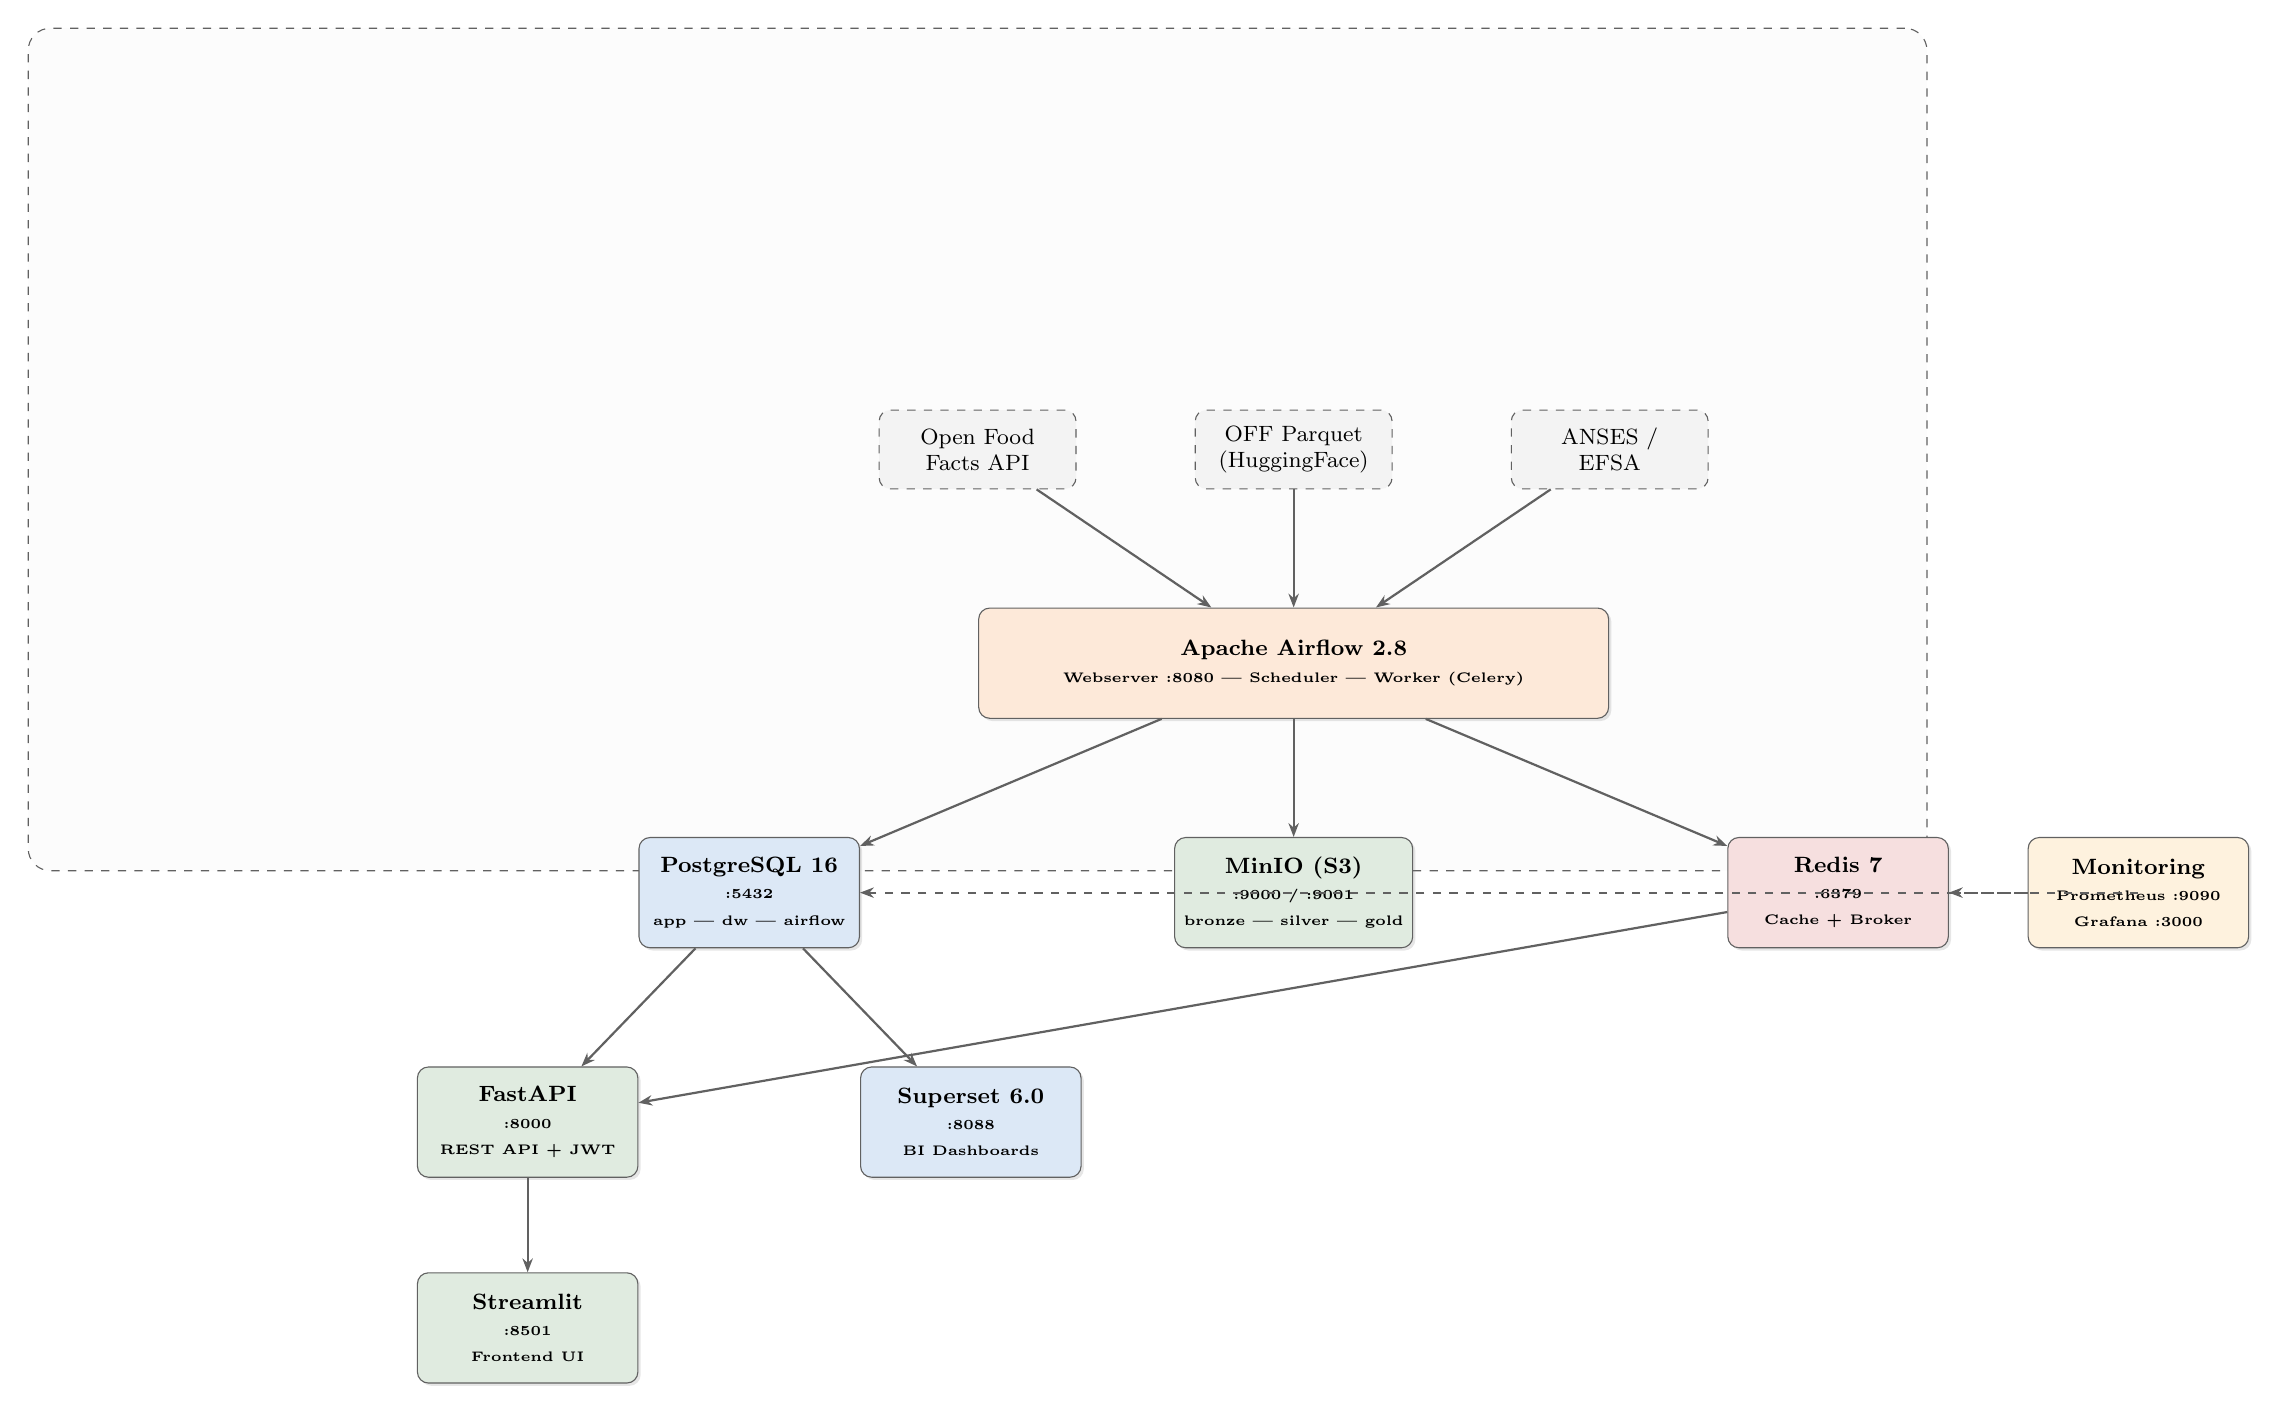
\begin{tikzpicture}[
  node distance=0.8cm and 1.2cm,
  service/.style={
    rectangle, rounded corners=4pt, draw=ntgray, fill=#1!15,
    minimum width=2.8cm, minimum height=1.4cm,
    font=\footnotesize\bfseries, align=center,
    drop shadow={shadow xshift=1pt, shadow yshift=-1pt, opacity=0.2}
  },
  service/.default=ntblue,
  ext/.style={
    rectangle, rounded corners=4pt, draw=ntgray, dashed,
    fill=ntlightgray!40, minimum width=2.5cm, minimum height=1cm,
    font=\footnotesize, align=center
  },
  arrow/.style={-{Stealth[length=5pt]}, thick, color=ntgray},
  label/.style={font=\tiny\color{ntgray}, midway},
]

% --- Row 1: External sources ---
\node[ext] (off) {Open Food\\Facts API};
\node[ext, right=1.5cm of off] (parquet) {OFF Parquet\\(HuggingFace)};
\node[ext, right=1.5cm of parquet] (anses) {ANSES /\\EFSA};

% --- Row 2: ETL Orchestration ---
\node[service=ntorange, below=1.5cm of parquet, minimum width=8cm] (airflow)
  {Apache Airflow 2.8\\{\tiny Webserver :8080 | Scheduler | Worker (Celery)}};

% --- Row 3: Storage ---
\node[service=ntblue, below left=1.5cm and 1.5cm of airflow] (postgres)
  {PostgreSQL 16\\{\tiny :5432}\\{\tiny app | dw | airflow}};
\node[service=ntgreen, below=1.5cm of airflow] (minio)
  {MinIO (S3)\\{\tiny :9000 / :9001}\\{\tiny bronze | silver | gold}};
\node[service=ntred, below right=1.5cm and 1.5cm of airflow] (redis)
  {Redis 7\\{\tiny :6379}\\{\tiny Cache + Broker}};

% --- Row 4: Applications ---
\node[service=ntgreen, below left=1.5cm and 0cm of postgres] (fastapi)
  {FastAPI\\{\tiny :8000}\\{\tiny REST API + JWT}};
\node[service=ntblue, below right=1.5cm and 0cm of postgres] (superset)
  {Superset 6.0\\{\tiny :8088}\\{\tiny BI Dashboards}};

% --- Row 5: Frontend ---
\node[service=ntgreen, below=1.2cm of fastapi] (streamlit)
  {Streamlit\\{\tiny :8501}\\{\tiny Frontend UI}};

% --- Monitoring ---
\node[service=ntgold, right=1cm of redis] (monitoring)
  {Monitoring\\{\tiny Prometheus :9090}\\{\tiny Grafana :3000}};

% --- Arrows ---
\draw[arrow] (off) -- (airflow);
\draw[arrow] (parquet) -- (airflow);
\draw[arrow] (anses) -- (airflow);
\draw[arrow] (airflow) -- (postgres);
\draw[arrow] (airflow) -- (minio);
\draw[arrow] (airflow) -- (redis);
\draw[arrow] (postgres) -- (fastapi);
\draw[arrow] (postgres) -- (superset);
\draw[arrow] (redis) -- (fastapi);
\draw[arrow] (fastapi) -- (streamlit);
\draw[arrow, dashed] (monitoring) -- (redis);
\draw[arrow, dashed] (monitoring) |- (postgres);

% --- Docker frame ---
\begin{scope}[on background layer]
  \node[draw=ntgray, dashed, rounded corners=8pt,
        fill=ntlightgray!10, inner sep=12pt,
        fit=(airflow)(postgres)(minio)(redis)(fastapi)(superset)
            (streamlit)(monitoring),
        label={[font=\small\bfseries\color{ntgray}]above:
          docker-compose.yml --- 15 services}] {};
\end{scope}

\end{tikzpicture}
\caption{\nutritrack{} system architecture --- Docker service overview}
\label{fig:arch-system}
\end{figure}


% =============================================================
% BLOCK 1: STEER A DATA PROJECT
% =============================================================
\chapter{Block 1 --- Steer a Data Project}
\label{ch:bloc1}

% -----------------------------------------------------------
\section{Need Analysis and Interview Grids}
\label{sec:e1}
{\small\evaluation{E1} | \competence{C1} | Deliverable: interview grids}

\subsection{Context and Business Need}

\nutritrack{} addresses a growing demand for personalized nutrition
tracking. The business need originates from three stakeholder groups:
(1)~end-users wishing to track their food intake and receive healthier
alternatives, (2)~nutritionists needing aggregated dietary data for
research and recommendations, and (3)~administrators managing the
platform and ensuring data quality.

The feasibility study identified \off{} as the primary data source --- a
collaborative, open-source database of food products with over 3~million
entries, including Nutri-Score ratings and detailed nutritional values.

\subsection{Interview Grid: Data Producers}

\begin{table}[H]
\centering
\caption{Interview grid --- Data producers}
\label{tab:grid-prod}
\begin{tabularx}{\textwidth}{C{0.5cm} L{7cm} L{2.5cm} L{3cm}}
\toprule
\textbf{\#} & \textbf{Question} & \textbf{Domain} & \textbf{Answer Type} \\
\midrule
1 & What food product databases do you maintain or contribute to? & Business activity & Source inventory \\
2 & How frequently is product information updated? & Characterization & Update cadence \\
3 & What metadata accompanies each product entry? & Metadata & Field inventory \\
4 & In what format is data stored or exported? & Storage format & Format list \\
5 & What access methods are available (REST API, bulk export, DB)? & Data access & Protocol list \\
6 & Are there rate limits or authentication requirements? & Access constraints & Technical limits \\
7 & What data quality issues have been observed? & Data quality & Defect categories \\
8 & How are contributions validated before publication? & Governance & Validation process \\
9 & Is there a data retention or archival policy? & Lifecycle & Retention rules \\
10 & Are there personal data elements? & \rgpd{} & Identification \\
\bottomrule
\end{tabularx}
\end{table}

\subsection{Interview Grid: Data Consumers}

\begin{table}[H]
\centering
\caption{Interview grid --- Data consumers}
\label{tab:grid-cons}
\begin{tabularx}{\textwidth}{C{0.5cm} L{7cm} L{2.5cm} L{3cm}}
\toprule
\textbf{\#} & \textbf{Question} & \textbf{Domain} & \textbf{Answer Type} \\
\midrule
1 & What nutritional analyses do you perform and what data is missing? & Business need & Gap analysis \\
2 & How do you currently search for product information? & Usage & User journey \\
3 & What level of nutritional detail is needed? & Granularity & Specification \\
4 & Do you need historical data to track reformulations? & Temporal analysis & Historization needs \\
5 & What aggregation level is useful? & Analytical granularity & Specification \\
6 & How should data be delivered? & Data access & Delivery preference \\
7 & What response time is acceptable? & Performance & SLA expectations \\
8 & Do you need to track individual meals (\rgpd{} implications)? & \rgpd{} & Consent requirements \\
9 & What accessibility accommodations are needed? & Accessibility & WCAG requirements \\
10 & Are there regulatory constraints on nutritional display? & Regulatory & Compliance \\
\bottomrule
\end{tabularx}
\end{table}

\subsection{Synthesis Note}

\subsubsection{Introduction --- Context, Stakes and Need Reformulation}

\textbf{Context:} Nutritional transparency is a growing societal concern in France and
across Europe, driven by public health policies (Plan National Nutrition Sant\'{e}) and
consumer demand for product transparency. The Open Food Facts project has assembled
over 3~million product entries collaboratively, but this data remains fragmented,
inconsistently formatted, and difficult to exploit for analytical or tracking purposes.

\textbf{Stakes:} The project's stakeholders require a centralized, clean and
governed data platform that transforms heterogeneous food product data into
actionable nutritional insights --- from personal meal tracking (end users) to
population-level dietary analysis (nutritionists) and infrastructure management
(administrators).

\textbf{Need reformulation:} Build an end-to-end data engineering platform that
(1)~collects food product data from 5 heterogeneous sources, (2)~cleans and
normalizes 798\,177 French products into a unified dataset of 777\,116 validated
records, (3)~stores data in a star-schema data warehouse with SCD historization,
(4)~exposes it via a secured REST API and a Streamlit frontend, and (5)~maintains
a MinIO-based data lake with medallion architecture and full \rgpd{} governance.

\subsubsection{Objectives and Scope}

The functional scope covers: data collection (5 source types), data cleaning and
aggregation (PySpark pipeline), relational storage (PostgreSQL 16 with 4 schemas),
analytical warehouse (star schema, 7 dimensions, 2 facts), data lake (MinIO medallion),
REST API (FastAPI, 8 endpoints, JWT), frontend (Streamlit, 4 roles), monitoring
(Prometheus + Grafana, 6 dashboards), and \rgpd{} compliance.

\subsubsection{Opportunity Study}

\textbf{Interview synthesis:} The data producer interviews (Table~\ref{tab:grid-prod})
revealed that the primary data source (\off{}) provides both a REST API and bulk
Parquet exports via HuggingFace. The data consumer interviews
(Table~\ref{tab:grid-cons}) confirmed the need for personalized nutrition tracking,
product comparison by Nutri-Score, and aggregated dietary trends.

\textbf{Benchmark:} A benchmark of existing solutions (Yuka, MyFitnessPal,
Cronometer) showed that none provide an open-source, self-hosted platform with
full data lineage and warehouse capabilities. The identified gap justified building
\nutritrack{} as a data engineering demonstration project.

\subsubsection{Feasibility Study}

\begin{itemize}[nosep]
  \item \textbf{Technical feasibility:} The \off{} API and Parquet dump are freely
        available. DuckDB can query the 4.2~GB Parquet file in $\sim$12 seconds.
        Docker Compose enables reproducible deployment of 15 services on a single
        machine.
  \item \textbf{Data feasibility:} 798\,177 French products with sufficient
        nutritional coverage (95\,\%+ on energy, proteins, fat, carbohydrates).
  \item \textbf{Organizational feasibility:} Solo developer project over 12 sprints;
        all tools are open-source with extensive documentation.
  \item \textbf{Financial feasibility:} Zero infrastructure cost (Docker, open-source);
        see CAPEX analysis in Section~\ref{sec:capex}.
\end{itemize}

\subsubsection{RICE Analysis}

\begin{table}[H]
\centering
\caption{RICE scoring for feature prioritization}
\label{tab:rice}
\begin{tabularx}{\textwidth}{L{3.5cm} C{1.2cm} C{1.2cm} C{1.2cm} C{1.2cm} C{1.5cm}}
\toprule
\textbf{Feature} & \textbf{Reach} & \textbf{Impact} & \textbf{Conf.} & \textbf{Effort} & \textbf{RICE} \\
\midrule
Product search + alternatives & 5 & 3 & 0.9 & 2 & 6.75 \\
ETL pipeline (full) & 4 & 3 & 1.0 & 3 & 4.00 \\
Star schema DW & 3 & 3 & 0.8 & 3 & 2.40 \\
Medallion data lake & 3 & 2 & 0.8 & 2 & 2.40 \\
Meal tracking + nutrition & 4 & 2 & 0.9 & 2 & 3.60 \\
SCD historization & 2 & 2 & 0.7 & 1 & 2.80 \\
Monitoring (Prometheus/Grafana) & 2 & 2 & 0.8 & 2 & 1.60 \\
RBAC governance & 3 & 2 & 0.9 & 1 & 5.40 \\
\bottomrule
\end{tabularx}
\end{table}

{\footnotesize \textbf{Scale:} Reach (1--5 stakeholder groups), Impact (1--3),
Confidence (0--1), Effort (1--3 sprints). RICE = (Reach $\times$ Impact
$\times$ Confidence) / Effort.}

\subsubsection{Pre-Project}

\textbf{Macro technical recommendations:}
\begin{itemize}[nosep]
  \item PostgreSQL 16 for both OLTP and OLAP (schema isolation), with migration
        path to dedicated OLAP engine at scale
  \item Apache Airflow 2.8 with CeleryExecutor for ETL orchestration
  \item PySpark 3.5 for distributed data cleaning on 800K+ records
  \item MinIO for S3-compatible object storage (medallion architecture)
  \item FastAPI for async REST API with JWT authentication
  \item Docker Compose for reproducible deployment
\end{itemize}

\textbf{Accessibility accommodations:}
\begin{itemize}[nosep]
  \item Streamlit UI with high-contrast Nutri-Score color coding
  \item All API documentation accessible via Swagger UI and ReDoc (keyboard-navigable)
  \item MkDocs documentation site with responsive layout and search
  \item Grafana dashboards with colorblind-friendly palettes
  \item Workstation adaptation: the platform runs entirely in Docker, deployable
        on any OS (macOS, Linux, Windows) without native dependencies
\end{itemize}

\textbf{\rgpd{} compliance actions:}
\begin{itemize}[nosep]
  \item Consent-based registration with explicit opt-in
  \item Data retention limits: user accounts 3 years, meal tracking 2 years
  \item SHA256 pseudonymization of user identifiers in the data warehouse
  \item Automated cleanup via \texttt{rgpd\_cleanup\_expired\_data()} PL/pgSQL function
  \item Personal data registry maintained (Table~\ref{tab:rgpd})
  \item No personal data in the data lake (gold layer uses anonymized aggregates)
  \item Data lake lifecycle rules: Bronze 90 days, backups 30 days
\end{itemize}


% -----------------------------------------------------------
\section{Data Topography, Architecture and Monitoring}
\label{sec:e2}
{\small\evaluation{E2} | \competence{C1, C2, C3, C4, C6} |
Deliverable: professional report}

\subsection{Data Topography (\competence{C2})}

\subsubsection{Semantics --- Business Glossary}

\begin{table}[H]
\centering
\caption{Business glossary --- Main objects}
\label{tab:glossary}
\begin{tabularx}{\textwidth}{L{2.5cm} L{6cm} L{4.5cm}}
\toprule
\textbf{Business Object} & \textbf{Description} & \textbf{Key Metadata} \\
\midrule
Product & Food product identified by barcode & barcode, name, brand, category, nutrition/100g, Nutri-Score, NOVA, Eco-Score \\
Brand & Manufacturer or distributor & name, parent company \\
Category & Hierarchical food classification & name, parent, level \\
User & User tracking their nutrition & UUID, email, role, goal, activity \\
Meal & Logged eating occasion & type, date, user\_id \\
Meal Item & Product within a meal & product\_id, quantity, computed nutrition \\
\bottomrule
\end{tabularx}
\end{table}

\subsubsection{Data Models}

The project uses multiple data modeling approaches adapted to each storage layer:

\begin{table}[H]
\centering
\caption{Data models by storage layer}
\label{tab:data-models-topo}
\begin{tabularx}{\textwidth}{L{2.5cm} L{2cm} L{3.5cm} L{4.5cm}}
\toprule
\textbf{Layer} & \textbf{Type} & \textbf{Model} & \textbf{Description} \\
\midrule
Operational (app) & Structured & Relational (3NF) & Products, brands, categories, users, meals, meal\_items with FK constraints \\
Data Warehouse (dw) & Structured & Star schema (Kimball) & 7 dimensions (time, product, brand, category, country, user, nutriscore) + 2 fact tables \\
Data Lake (bronze) & Semi-structured & Raw files & JSON (API, scraping), Parquet (bulk export), unmodified from source \\
Data Lake (silver) & Semi-structured & Cleaned Parquet & Unified schema, validated and deduplicated \\
Data Lake (gold) & Semi-structured & Analytical Parquet & Pre-aggregated datasets for analytics consumption \\
\bottomrule
\end{tabularx}
\end{table}

\subsubsection{Treatments and Data Flows --- Flux Matrix}

\begin{figure}[H]
\centering
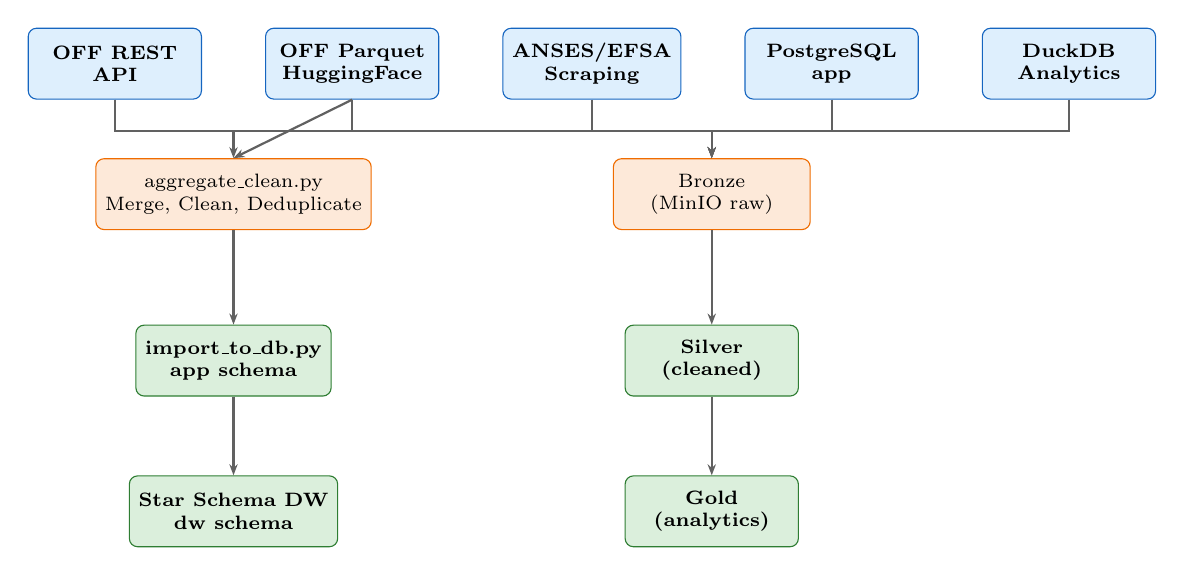
\begin{tikzpicture}[
  node distance=0.6cm,
  source/.style={
    rectangle, rounded corners=3pt, draw=ntblue, fill=ntlightblue!30,
    minimum width=2.2cm, minimum height=0.9cm,
    font=\scriptsize\bfseries, align=center
  },
  process/.style={
    rectangle, rounded corners=3pt, draw=ntorange, fill=ntorange!15,
    minimum width=2.5cm, minimum height=0.9cm,
    font=\scriptsize, align=center
  },
  target/.style={
    rectangle, rounded corners=3pt, draw=ntgreen, fill=ntlightgreen!40,
    minimum width=2.2cm, minimum height=0.9cm,
    font=\scriptsize\bfseries, align=center
  },
  arr/.style={-{Stealth[length=4pt]}, thick, color=ntgray},
]

% Sources
\node[source] (api) {OFF REST\\API};
\node[source, right=0.8cm of api] (pq) {OFF Parquet\\HuggingFace};
\node[source, right=0.8cm of pq] (scrap) {ANSES/EFSA\\Scraping};
\node[source, right=0.8cm of scrap] (db) {PostgreSQL\\app};
\node[source, right=0.8cm of db] (duck) {DuckDB\\Analytics};

% Processing
\node[process, below=1.2cm of $(api)!0.5!(pq)$] (agg) {aggregate\_clean.py\\Merge, Clean, Deduplicate};
\node[process, below=1.2cm of $(scrap)!0.5!(db)$] (bronze) {Bronze\\(MinIO raw)};

% Targets
\node[target, below=1.2cm of agg] (import) {import\_to\_db.py\\app schema};
\node[target, below=1.2cm of bronze] (silverT) {Silver\\(cleaned)};

\node[target, below=1cm of import] (dw) {Star Schema DW\\dw schema};
\node[target, below=1cm of silverT] (goldT) {Gold\\(analytics)};

% Arrows from sources
\draw[arr] (api.south) -- ++(0,-0.4) -| (agg.north);
\draw[arr] (pq.south) -- (agg.north);
\draw[arr] (scrap.south) -- ++(0,-0.4) -| (bronze.north);
\draw[arr] (db.south) -- ++(0,-0.4) -| (bronze.north);
\draw[arr] (duck.south) -- ++(0,-0.4) -| (bronze.north);
\draw[arr] (api.south) -- ++(0,-0.4) -| (bronze.north);
\draw[arr] (pq.south) -- ++(0,-0.4) -| (bronze.north);

% Processing to targets
\draw[arr] (agg) -- (import);
\draw[arr] (bronze) -- (silverT);
\draw[arr] (import) -- (dw);
\draw[arr] (silverT) -- (goldT);

\end{tikzpicture}
\caption{Data pipeline --- From sources to analytical layers}
\label{fig:data-pipeline}
\end{figure}


\subsubsection{Access and Usage Conditions}

\begin{table}[H]
\centering
\caption{Data access and usage conditions}
\label{tab:access-conditions}
\begin{tabularx}{\textwidth}{L{2.5cm} L{2.5cm} L{3cm} L{4.5cm}}
\toprule
\textbf{Data Source} & \textbf{Access Method} & \textbf{License} & \textbf{Conditions} \\
\midrule
OFF REST API & HTTP GET & ODbL v1.0 & Rate limit: 100 req/min; User-Agent required \\
OFF Parquet & HuggingFace download & ODbL v1.0 & 4.2~GB bulk file; updated weekly \\
ANSES/EFSA & Web scraping & Public domain & Respectful crawling; robots.txt compliance \\
PostgreSQL (app) & SQL connection & Internal & Authentication required; role-based access \\
DuckDB analytics & Embedded SQL & Internal & Read-only on Parquet files \\
\bottomrule
\end{tabularx}
\end{table}

\textbf{Data availability:} The OFF dataset is available 24/7 via both API and bulk
download. ANSES reference values are static and cached locally. Internal PostgreSQL
data is available whenever the Docker Compose stack is running.

\subsection{Technical Architecture Study (\competence{C3})}

\subsubsection{Functional Analysis}

The system must: (1)~collect food product data from 5 heterogeneous
sources, (2)~clean, normalize and deduplicate the data, (3)~store
structured data in PostgreSQL, (4)~expose data via a secured REST API,
(5)~provide a nutrition tracking interface, and (6)~maintain a data lake
with medallion architecture.

\subsubsection{Non-Functional Requirements}

\begin{table}[H]
\centering
\caption{Non-functional requirements and chosen solutions}
\label{tab:nonfunc}
\begin{tabularx}{\textwidth}{L{2.5cm} L{4cm} L{6cm}}
\toprule
\textbf{Constraint} & \textbf{Requirement} & \textbf{Solution} \\
\midrule
Performance & Product search $<$~1s & GIN full-text index, connection pooling (pool\_size=10) \\
Scalability & Handle 3M+ products & DuckDB for in-memory analytics on Parquet \\
Reliability & Zero data loss & Airflow retries (2--3 attempts), audit log \\
Security & No plaintext passwords & bcrypt hashing, JWT HS256, RBAC \\
Availability & Health monitoring & Docker healthchecks, Airflow UI, \texttt{/health} endpoint \\
\bottomrule
\end{tabularx}
\end{table}

\subsubsection{Architecture Decisions}

\begin{table}[H]
\centering
\caption{Key architecture decisions}
\label{tab:arch-decisions}
\begin{tabularx}{\textwidth}{L{3.5cm} L{3cm} L{6.5cm}}
\toprule
\textbf{Decision} & \textbf{Choice} & \textbf{Rationale} \\
\midrule
OLTP/OLAP DB & Single PostgreSQL & Simplifies deployment; adequate at current scale. \textit{Alternatives: MySQL (less analytical), ClickHouse (overkill at this scale)} \\
ETL orchestrator & Apache Airflow & Industry standard, DAG-based, web UI, Celery. \textit{Alternatives: Prefect (less mature), Luigi (no web UI)} \\
ETL engine & PySpark 3.5 & Distributed cleaning on 800K+ rows, cluster-ready. \textit{Alternatives: pandas (memory limits), dbt (SQL-only)} \\
Data lake storage & MinIO (S3) & Open-source, self-hosted, AWS S3-compatible API. \textit{Alternatives: HDFS (heavy), AWS S3 (cost)} \\
API framework & FastAPI (async) & Native async support, auto-generated OpenAPI docs. \textit{Alternatives: Flask (sync), Django REST (heavy)} \\
Big data & DuckDB & Direct Parquet reads, SQL interface, zero config. \textit{Alternatives: Spark SQL (heavy), Trino (complex)} \\
Authentication & JWT + bcrypt & Stateless, scalable, standard REST. \textit{Alternatives: OAuth2 (complex), session-based (stateful)} \\
DW approach & Bottom-up & Fast value delivery; datamarts first. \textit{Alternative: top-down (Inmon, longer initial setup)} \\
\bottomrule
\end{tabularx}
\end{table}

\subsubsection{\rgpd{} Compliance}

\begin{table}[H]
\centering
\caption{Personal data registry (excerpt)}
\label{tab:rgpd}
\begin{tabularx}{\textwidth}{L{2.8cm} L{2.5cm} L{2cm} L{5.5cm}}
\toprule
\textbf{Category} & \textbf{Legal Basis} & \textbf{Retention} & \textbf{Security Measures} \\
\midrule
User account & Consent (Art.~6.1.a) & 3 years & bcrypt hashing, encrypted storage \\
User profile & Consent (Art.~6.1.a) & 3 years & Pseudonymized (SHA256) in analytics \\
Meal tracking & Consent (Art.~6.1.a) & 2 years & Associated with UUID, deletable on request \\
Product data & Legitimate interest (Art.~6.1.f) & Indefinite & Public data \\
\bottomrule
\end{tabularx}
\end{table}

\textbf{Sorting and deletion procedures:}
\begin{itemize}[nosep]
  \item \texttt{rgpd\_cleanup\_expired\_data()}: PL/pgSQL function automating
        deletion of meals $>$~2 years and deactivation of accounts past
        retention
  \item Data lake lifecycle rules: Bronze expires at 90 days,
        backups at 30 days
\end{itemize}

\begin{figure}[H]
\centering
\begin{tikzpicture}[
  node distance=0.7cm and 1.5cm,
  step/.style={
    rectangle, rounded corners=4pt, draw=ntblue, fill=ntlightblue!20,
    minimum width=3.2cm, minimum height=0.9cm,
    font=\scriptsize\bfseries, align=center
  },
  decision/.style={
    diamond, draw=ntorange, fill=ntorange!15,
    minimum width=1.5cm, minimum height=1cm,
    font=\scriptsize, aspect=2, align=center
  },
  arr/.style={-{Stealth[length=4pt]}, thick, color=ntgray},
]

% Steps
\node[step] (collect) {Data collection\\{\tiny with consent}};
\node[step, right=2cm of collect] (registry) {Register in\\\rgpd{} registry};
\node[step, below=1cm of registry] (hash) {Pseudonymization\\{\tiny SHA256 in DW}};
\node[step, below=1cm of hash] (retention) {Retention\\check};
\node[decision, below=1cm of retention] (expired) {Expired?};
\node[step, below left=1cm and 1.5cm of expired] (keep) {Keep\\{\tiny controlled access}};
\node[step, below right=1cm and 1.5cm of expired] (delete) {Delete /\\Deactivate};

% Arrows
\draw[arr] (collect) -- (registry);
\draw[arr] (registry) -- (hash);
\draw[arr] (hash) -- (retention);
\draw[arr] (retention) -- (expired);
\draw[arr] (expired) -- node[font=\tiny, left] {No} (keep);
\draw[arr] (expired) -- node[font=\tiny, right] {Yes} (delete);

\end{tikzpicture}
\caption{\rgpd{} process --- From consent to deletion}
\label{fig:rgpd-process}
\end{figure}

\subsubsection{Eco-Responsibility Strategy}

Following the French RGESN framework:
\begin{enumerate}[nosep]
  \item \textbf{Efficient queries}: DuckDB processes 3M+ products without full loading
  \item \textbf{Minimal transfers}: API pagination, delta ETL
  \item \textbf{Lifecycle}: Bronze expires at 90 days, backups at 30 days
  \item \textbf{Lightweight containers}: Alpine images (PostgreSQL, Redis)
  \item \textbf{Batch processing}: ETL during off-peak hours (02:00--06:00 UTC)
\end{enumerate}

\subsubsection{Risks and Costs}
\label{sec:capex}

\textbf{CAPEX / Infrastructure Cost Analysis:}

\begin{table}[H]
\centering
\caption{Infrastructure cost comparison --- On-premise (Docker) vs.\ Cloud (AWS)}
\label{tab:capex}
\begin{tabularx}{\textwidth}{L{4cm} C{2.5cm} C{2.5cm} L{3.5cm}}
\toprule
\textbf{Component} & \textbf{Docker (actual)} & \textbf{AWS equivalent} & \textbf{Notes} \\
\midrule
Compute (15 services) & 0~EUR & $\sim$2\,400~EUR/yr & t3.xlarge (4 vCPU, 16~GB) \\
PostgreSQL 16 & 0~EUR & $\sim$1\,800~EUR/yr & RDS db.t3.medium \\
Object storage (6~GB) & 0~EUR & $\sim$50~EUR/yr & S3 Standard \\
ETL orchestration & 0~EUR & $\sim$2\,400~EUR/yr & MWAA (managed Airflow) \\
Monitoring & 0~EUR & $\sim$1\,200~EUR/yr & CloudWatch + Grafana Cloud \\
Networking / data transfer & 0~EUR & $\sim$150~EUR/yr & Outbound data transfer \\
\midrule
\textbf{Total annual} & \textbf{0~EUR} & \textbf{$\sim$8\,000~EUR/yr} & \\
\bottomrule
\end{tabularx}
\end{table}

\textbf{Licensing:} All software components are open-source (PostgreSQL, Airflow,
MinIO, FastAPI, PySpark, DuckDB, Streamlit, Prometheus, Grafana, Redis).
Total licensing cost: 0~EUR.

\textbf{Risk Evaluation per Phase:}

\begin{table}[H]
\centering
\caption{Risk evaluation by project phase}
\label{tab:risks}
\begin{tabularx}{\textwidth}{C{1cm} L{3.5cm} C{1.2cm} C{1.2cm} L{4.5cm}}
\toprule
\textbf{Phase} & \textbf{Risk} & \textbf{Prob.} & \textbf{Impact} & \textbf{Mitigation} \\
\midrule
1 & Incomplete requirements & Medium & High & Interview grids with all stakeholder groups; iterative validation \\
2 & API rate limiting / data unavailability & Medium & High & Multiple source strategy (API + Parquet + scraping); local caching \\
2 & Data quality issues in OFF & High & Medium & 7-rule cleaning pipeline; 6 data quality checks; cleaning report \\
3 & Schema evolution breaking API & Low & High & Versioned API (\texttt{/api/v1/}); migration scripts \\
4 & ETL failures blocking analytics & Medium & High & Airflow retries (2--3 attempts); MailHog alerting; SLA monitoring \\
4 & SCD complexity causing data inconsistencies & Medium & Medium & Unit tests for SCD logic; \texttt{IS DISTINCT FROM} for NULL handling \\
5 & MinIO storage exhaustion & Low & Medium & Lifecycle rules (bronze 90d, backups 30d); storage monitoring \\
6 & Integration issues between services & Medium & Medium & Docker Compose healthchecks; end-to-end pipeline testing \\
\bottomrule
\end{tabularx}
\end{table}

\subsection{Technical Monitoring (\competence{C4})}

\textbf{Theme:} Apache Airflow --- ETL orchestration and observability.\\
\textbf{Schedule:} Minimum 1h/week reviewing DAG logs, pipeline health
and data quality metrics via the Airflow web interface (port 8080).\\
\textbf{Aggregation tools:} Airflow Web UI, \texttt{extraction\_log}
table, JSON cleaning report.

\textbf{Technology watch newsletter:} A dedicated technology watch
document (\texttt{docs/veille\_technologique.md}) is maintained as part
of the C4 competency. It covers the monitoring theme in depth, including
tool comparisons, emerging practices in ETL observability, and weekly
review summaries. The newsletter is published via the MkDocs
documentation site (see Section~\ref{sec:cicd-docs}).

\subsection{Project Supervision (\competence{C6})}

Tracking tools: Airflow Web UI, \texttt{extraction\_log} table,
standardized Makefile. Indicators updated throughout the project:
records extracted/loaded/rejected, completeness percentage per column,
DAG success rate.

\textbf{Historical activity log:} The \texttt{app.etl\_activity\_log}
table (see Section~\ref{sec:c16}) records structured log entries with
alert categories (\texttt{CRITICAL}, \texttt{WARNING}, \texttt{INFO})
for every ETL operation. The table is seeded with historical data
spanning 14 days of project activity (migration
\texttt{002\_seed\_etl\_activity\_log.sql}), demonstrating that
indicators have been tracked throughout the project lifecycle.


% -----------------------------------------------------------
\section{Project Planning and Communication}
\label{sec:e3}
{\small\evaluation{E3} | \competence{C5, C6, C7} |
Deliverable: kickoff meeting simulation}

\subsection{Project Roadmap (\competence{C5})}

\begin{table}[H]
\centering
\caption{Project roadmap in 6 phases}
\label{tab:roadmap}
\begin{tabularx}{\textwidth}{L{1cm} L{2cm} L{3cm} L{5cm} C{1.5cm}}
\toprule
\textbf{Phase} & \textbf{Duration} & \textbf{Deliverables} & \textbf{Milestone} & \textbf{SP} \\
\midrule
1 & 2 weeks & Grids, feasibility & Architecture validated & 21 \\
2 & 3 weeks & 5 extraction scripts & Pipeline operational & 24 \\
3 & 2 weeks & DB, REST API & API functional & 21 \\
4 & 2 weeks & Star schema, ETL & DW populated & 21 \\
5 & 2 weeks & MinIO, medallion & Lake operational & 16 \\
6 & 1 week & Streamlit, tests & Platform ready & 13 \\
\bottomrule
\end{tabularx}
\end{table}

\textbf{Effort weighting method:} Fibonacci story points via team
estimation (poker planning). Each user story is estimated by the team during
sprint planning using the Fibonacci sequence (1, 2, 3, 5, 8, 13). The total
of 116 story points is distributed across 6 phases as shown above.

\subsection{Team Composition and Budget (\competence{C5})}

\begin{table}[H]
\centering
\caption{Team composition and required skills}
\label{tab:team}
\begin{tabularx}{\textwidth}{L{3cm} L{3.5cm} L{3cm} C{2cm}}
\toprule
\textbf{Role} & \textbf{Skills Required} & \textbf{Phases Active} & \textbf{Allocation} \\
\midrule
Project Lead / Data Engineer & Python, SQL, ETL, Docker, Airflow & All (1--6) & 100\,\% \\
Data Architect & PostgreSQL, star schema, SCD & Phases 1, 3, 4 & 50\,\% \\
Backend Developer & FastAPI, JWT, REST API design & Phases 3, 6 & 50\,\% \\
DevOps Engineer & Docker, CI/CD, monitoring & Phases 1, 5, 6 & 25\,\% \\
\bottomrule
\end{tabularx}
\end{table}

\textbf{Budget allocation:} In this project context (certification demonstration),
all roles are fulfilled by the candidate. The theoretical budget based on market
rates would be approximately 45\,000~EUR for 3 months (1 FTE senior data engineer
at 550~EUR/day $\times$ 60 days + 0~EUR infrastructure).

\subsection{Gantt Calendar (\competence{C5})}

\begin{figure}[H]
\centering
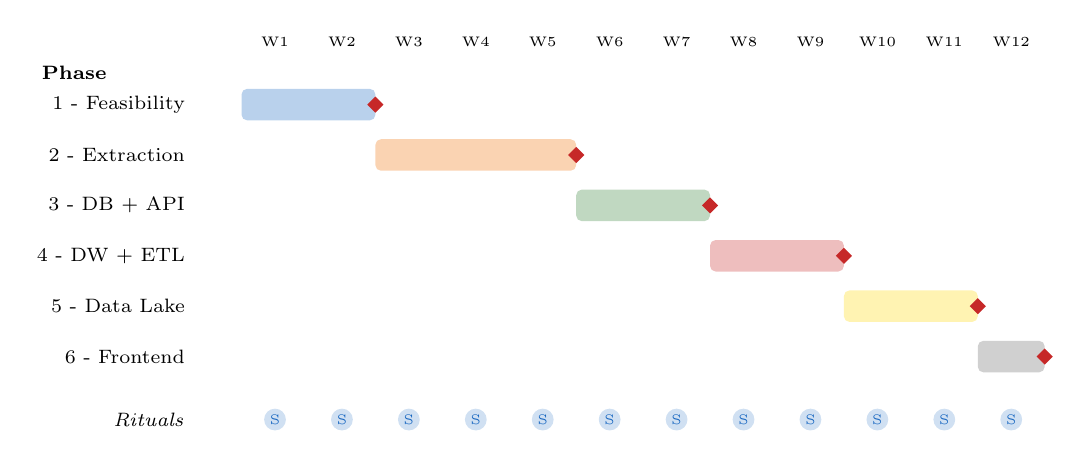
\begin{tikzpicture}[
  x=0.85cm, y=0.8cm,
  phase/.style={fill=#1!30, draw=#1!60, rounded corners=2pt, minimum height=0.55cm},
]
% Header
\node[font=\scriptsize\bfseries] at (-2, 0.5) {Phase};
\foreach \w in {1,...,12} {
  \node[font=\tiny] at (\w, 1) {W\w};
}

% Phase bars
\node[font=\scriptsize, anchor=east] at (-0.2, 0) {1 - Feasibility};
\fill[ntblue!30, rounded corners=2pt] (0.5,-0.25) rectangle (2.5,0.25);

\node[font=\scriptsize, anchor=east] at (-0.2, -0.8) {2 - Extraction};
\fill[ntorange!30, rounded corners=2pt] (2.5,-1.05) rectangle (5.5,-0.55);

\node[font=\scriptsize, anchor=east] at (-0.2, -1.6) {3 - DB + API};
\fill[ntgreen!30, rounded corners=2pt] (5.5,-1.85) rectangle (7.5,-1.35);

\node[font=\scriptsize, anchor=east] at (-0.2, -2.4) {4 - DW + ETL};
\fill[ntred!30, rounded corners=2pt] (7.5,-2.65) rectangle (9.5,-2.15);

\node[font=\scriptsize, anchor=east] at (-0.2, -3.2) {5 - Data Lake};
\fill[gold!30, rounded corners=2pt] (9.5,-3.45) rectangle (11.5,-2.95);

\node[font=\scriptsize, anchor=east] at (-0.2, -4.0) {6 - Frontend};
\fill[ntgray!30, rounded corners=2pt] (11.5,-4.25) rectangle (12.5,-3.75);

% Milestones
\node[font=\tiny\color{ntred}, diamond, fill=ntred, inner sep=1.5pt] at (2.5, 0) {};
\node[font=\tiny\color{ntred}, diamond, fill=ntred, inner sep=1.5pt] at (5.5, -0.8) {};
\node[font=\tiny\color{ntred}, diamond, fill=ntred, inner sep=1.5pt] at (7.5, -1.6) {};
\node[font=\tiny\color{ntred}, diamond, fill=ntred, inner sep=1.5pt] at (9.5, -2.4) {};
\node[font=\tiny\color{ntred}, diamond, fill=ntred, inner sep=1.5pt] at (11.5, -3.2) {};
\node[font=\tiny\color{ntred}, diamond, fill=ntred, inner sep=1.5pt] at (12.5, -4.0) {};

% Rituals bar
\node[font=\scriptsize, anchor=east] at (-0.2, -5.0) {\textit{Rituals}};
\foreach \w in {1,...,12} {
  \node[font=\tiny\color{ntblue}, circle, fill=ntblue!20, inner sep=1pt] at (\w, -5.0) {S};
}

\end{tikzpicture}
\caption{Gantt calendar --- 12-week sprint plan with milestones (diamonds) and weekly standups (S)}
\label{fig:gantt}
\end{figure}

\textbf{Collaborative rituals:}
\begin{itemize}[nosep]
  \item \textbf{Daily standup} (15 min): progress, blockers, plan for the day
  \item \textbf{Sprint planning} (1h, bi-weekly): backlog grooming, poker planning estimation
  \item \textbf{Sprint review} (30 min, bi-weekly): demo of completed work to stakeholders
  \item \textbf{Sprint retrospective} (30 min, bi-weekly): what went well, what to improve
  \item \textbf{Phase milestone demo} (1h, end of each phase): formal milestone validation
\end{itemize}

\textbf{Tracking tool configuration:} GitHub Projects board with columns
(Backlog, Sprint, In Progress, Review, Done). Issues tagged with competency
labels (C1--C21) and phase labels. Board accessible to all stakeholders via
the repository at \url{https://github.com/Reetika12795/NutriTrack}.

\subsection{Communication Strategy (\competence{C7})}

\begin{table}[H]
\centering
\caption{Communication plan}
\label{tab:comms}
\begin{tabularx}{\textwidth}{L{2.5cm} L{2.5cm} L{2cm} L{2cm} L{3.5cm}}
\toprule
\textbf{Communication} & \textbf{Audience} & \textbf{Format} & \textbf{Frequency} & \textbf{Content} \\
\midrule
Sprint kickoff & All stakeholders & Presentation & Bi-weekly & Sprint goals \\
Progress update & Sponsor & Email & Weekly & Milestones, blockers \\
Technical demo & Team + nutritionists & Live demo & End of phase & Features, quality \\
API docs & Developers & OpenAPI & Continuous & Endpoints, auth \\
Final delivery & Jury & Oral + report & End of project & Full demo \\
\bottomrule
\end{tabularx}
\end{table}

\textbf{User documentation:} Production of user documentation is planned in
Phase~6 and includes: MkDocs technical documentation site (auto-deployed via
GitHub Actions), OpenAPI/Swagger interactive API docs, and a quick-start guide
in the repository README.

\textbf{End-user onboarding plan:}
\begin{enumerate}[nosep]
  \item \textbf{Onboarding session 1} (Phase 6, Week 11): Nutritionists ---
        walkthrough of Streamlit dashboard, data warehouse datamarts, and
        Superset BI dashboards
  \item \textbf{Onboarding session 2} (Phase 6, Week 12): Administrators ---
        Airflow DAG management, MinIO console, Grafana monitoring, backup procedures
  \item \textbf{Self-service documentation}: MkDocs site with architecture overview,
        API reference, and troubleshooting guide
\end{enumerate}

\textbf{Feedback collection process:}
\begin{itemize}[nosep]
  \item \textbf{Sprint reviews}: Stakeholder feedback collected during bi-weekly demos;
        action items logged in GitHub Issues
  \item \textbf{Phase milestone surveys}: Short feedback form (5 questions) distributed
        after each phase demo to assess satisfaction and identify gaps
  \item \textbf{Post-deployment feedback}: GitHub Issues template for bug reports and
        feature requests, integrated into sprint backlog
  \item \textbf{Continuous}: Slack channel for real-time questions and feedback
\end{itemize}


% =============================================================
% BLOCK 2: DATA COLLECTION, STORAGE AND SHARING
% =============================================================
\chapter{Block 2 --- Data Collection, Storage and Sharing}
\label{ch:bloc2}

% -----------------------------------------------------------
\section{Extraction Scripts (\competence{C8})}
\label{sec:c8}
{\small\evaluation{E4} | 5 extraction scripts from heterogeneous sources}

All extraction scripts follow a consistent structure: entry point
(\texttt{main()}), dependency initialization, external connection
configuration, business logic rules, error handling, and result saving.
All are versioned on Git.

\subsection{Source 1: REST API}

\textbf{File:} \texttt{scripts/extract\_off\_api.py}

\begin{lstlisting}[language=Python, caption={REST API extraction --- Open Food Facts}]
def extract_products_by_category(
    category: str, max_pages: int = 10, page_size: int = 50
) -> list[dict]:
    all_products = []
    for page in range(1, max_pages + 1):
        products = search_products(category, page=page,
                                   page_size=page_size)
        if not products:
            break
        all_products.extend(products)
        time.sleep(0.6)  # Rate limiting
    return all_products
\end{lstlisting}

\subsection{Source 2: Parquet File + DuckDB}

\textbf{File:} \texttt{scripts/extract\_off\_parquet.py}\\
Result: 798\,177 French products extracted in $\sim$12 seconds from a
4.1~GB Parquet file.

\begin{lstlisting}[language=SQL, caption={DuckDB query --- Parquet extraction with nested structures}]
SELECT
    code AS barcode, product_name,
    (SELECT n.per_100g FROM UNNEST(nutriments) n
     WHERE n.name = 'energy-kcal') AS energy_kcal,
    (SELECT n.per_100g FROM UNNEST(nutriments) n
     WHERE n.name = 'proteins') AS proteins_g,
    nutriscore_grade, nova_group
FROM read_parquet('food.parquet')
WHERE code IS NOT NULL
  AND list_contains(countries_tags, 'en:france')
ORDER BY completeness DESC;
\end{lstlisting}

\subsection{Source 3: Web Scraping}

\textbf{File:} \texttt{scripts/extract\_scraping.py}\\
BeautifulSoup extraction of HTML tables from ANSES and EFSA with
fallback to EU Regulation~1169/2011 reference values.

\subsection{Source 4: PostgreSQL Database}

\textbf{File:} \texttt{scripts/extract\_from\_db.py}\\
Product extraction with brand and category joins from the operational
schema, output in Parquet and CSV.

\subsection{Source 5: Big Data System (DuckDB Analytics)}

\textbf{File:} \texttt{scripts/extract\_duckdb.py}\\
Complex analytical queries on the full 3M+ product dataset, including
Nutri-Score distribution by country.


% -----------------------------------------------------------
\section{SQL Queries (\competence{C9})}
\label{sec:c9}

\textbf{File:} \texttt{sql/queries/analytical\_queries.sql} (7 queries)

\begin{lstlisting}[language=SQL, caption={Query 2 --- Full-text search with Nutri-Score filter}]
SELECT p.barcode, p.product_name, b.brand_name,
       p.nutriscore_grade,
       ts_rank(to_tsvector('french', p.product_name),
               plainto_tsquery('french', 'chocolat noir'))
               AS relevance
FROM app.products p
LEFT JOIN app.brands b ON p.brand_id = b.brand_id
WHERE to_tsvector('french', p.product_name)
      @@ plainto_tsquery('french', 'chocolat noir')
  AND p.nutriscore_grade IN ('A', 'B', 'C')
ORDER BY relevance DESC LIMIT 20;
\end{lstlisting}

\textbf{Optimization:} GIN index on \texttt{to\_tsvector('french',
product\_name)} for sub-second search across 100\,000+ products.


% -----------------------------------------------------------
\section{Aggregation and Cleaning Pipeline (\competence{C10})}
\label{sec:c10}

\textbf{File:} \texttt{scripts/aggregate\_clean.py}

\begin{figure}[H]
\centering
\begin{tikzpicture}[
  node distance=0.5cm,
  step/.style={
    rectangle, rounded corners=3pt, draw=ntblue, fill=ntlightblue!20,
    minimum width=6cm, minimum height=0.7cm,
    font=\scriptsize, align=center
  },
  arr/.style={-{Stealth[length=4pt]}, thick, color=ntgray},
]
\node[step] (s1) {Standardize columns (30+ mappings)};
\node[step, below=of s1] (s2) {Clean barcodes (8--14 digits)};
\node[step, below=of s2] (s3) {Clean text (normalize, remove control characters)};
\node[step, below=of s3] (s4) {Remove entries without product\_name};
\node[step, below=of s4] (s5) {Convert kJ $\rightarrow$ kcal if kcal missing};
\node[step, below=of s5] (s6) {Validate numeric ranges (energy $\leq$ 1000, etc.)};
\node[step, below=of s6] (s7) {Normalize Nutri-Score (A--E) and NOVA (1--4)};
\node[step, below=of s7] (s8) {Deduplicate by barcode (keep most complete)};

\foreach \i/\j in {s1/s2, s2/s3, s3/s4, s4/s5, s5/s6, s6/s7, s7/s8} {
  \draw[arr] (\i) -- (\j);
}

% Input/output labels
\node[font=\scriptsize\bfseries\color{ntgreen}, above=0.3cm of s1]
  {798\,177 raw products (5 sources)};
\node[font=\scriptsize\bfseries\color{ntgreen}, below=0.3cm of s8]
  {777\,126 clean products (97.4\,\% retention)};
\end{tikzpicture}
\caption{Data cleaning pipeline}
\label{fig:cleaning-pipeline}
\end{figure}


% -----------------------------------------------------------
\section{Database Modeling and \rgpd{} (\competence{C11})}
\label{sec:c11}

\subsection{Conceptual Data Model (MCD)}

\begin{figure}[H]
\centering
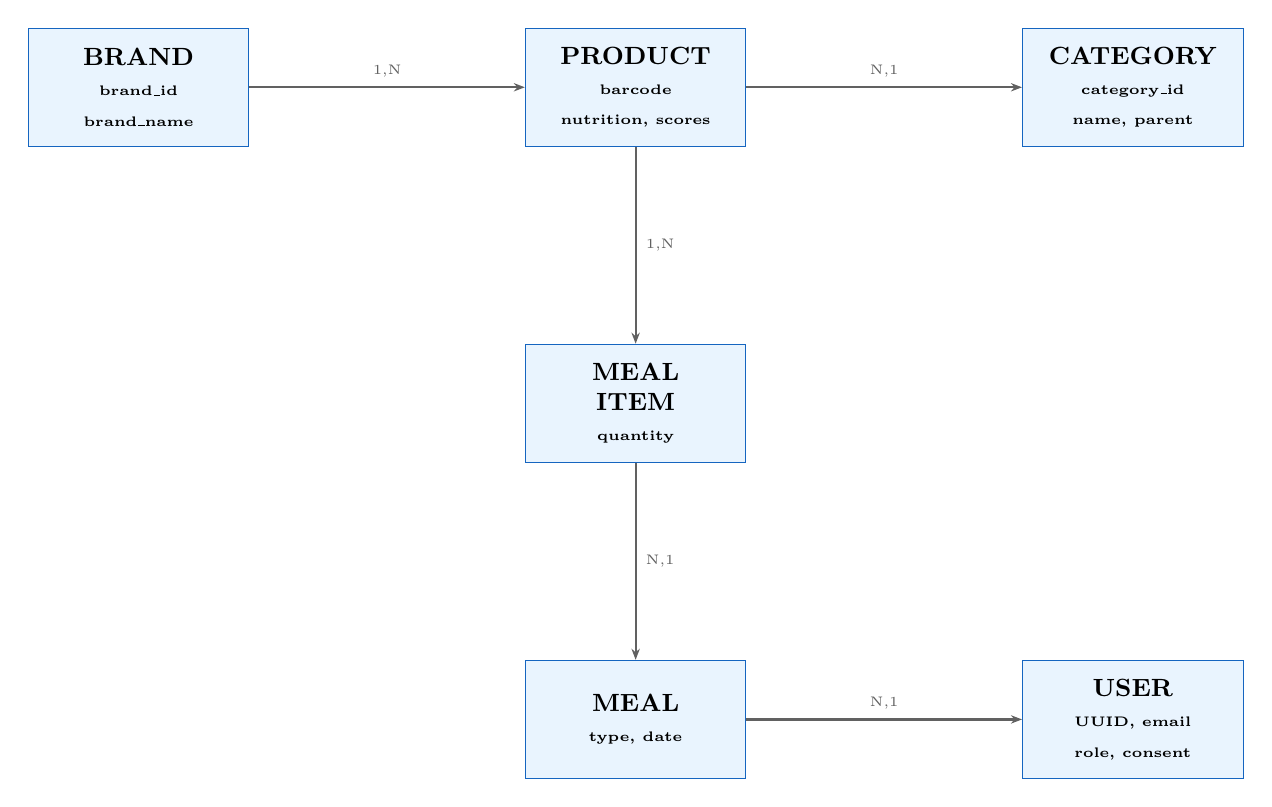
\begin{tikzpicture}[
  entity/.style={
    rectangle, draw=ntblue, fill=ntlightblue!20,
    minimum width=2.8cm, minimum height=1.5cm,
    font=\small\bfseries, align=center
  },
  rel/.style={
    diamond, draw=ntorange, fill=ntorange!15,
    minimum width=1cm, minimum height=0.8cm,
    font=\tiny, aspect=2
  },
  arr/.style={-{Stealth[length=4pt]}, thick, color=ntgray},
  card/.style={font=\tiny\color{ntgray}, midway},
]

\node[entity] (brand) {BRAND\\{\tiny brand\_id}\\{\tiny brand\_name}};
\node[entity, right=3.5cm of brand] (product) {PRODUCT\\{\tiny barcode}\\{\tiny nutrition, scores}};
\node[entity, right=3.5cm of product] (cat) {CATEGORY\\{\tiny category\_id}\\{\tiny name, parent}};

\node[entity, below=2.5cm of product] (mealitem) {MEAL\\ITEM\\{\tiny quantity}};
\node[entity, below=2.5cm of mealitem] (meal) {MEAL\\{\tiny type, date}};
\node[entity, right=3.5cm of meal] (user) {USER\\{\tiny UUID, email}\\{\tiny role, consent}};

% Relations
\draw[arr] (brand) -- node[card, above] {1,N} (product);
\draw[arr] (product) -- node[card, above] {N,1} (cat);
\draw[arr] (product) -- node[card, right] {1,N} (mealitem);
\draw[arr] (mealitem) -- node[card, right] {N,1} (meal);
\draw[arr] (meal) -- node[card, above] {N,1} (user);

\end{tikzpicture}
\caption{Conceptual Data Model (MCD)}
\label{fig:mcd}
\end{figure}

\subsection{Logical Data Model (MLD)}

The logical model translates the conceptual model into relational tables with
primary keys, foreign keys, and data types, without implementation-specific
details:

\begin{table}[H]
\centering
\caption{Logical Data Model (MLD) --- Table structure}
\label{tab:mld}
\begin{tabularx}{\textwidth}{L{2.5cm} L{10cm}}
\toprule
\textbf{Table} & \textbf{Attributes} \\
\midrule
BRAND & \underline{brand\_id} (PK), brand\_name (VARCHAR, NOT NULL) \\
CATEGORY & \underline{category\_id} (PK), category\_name (VARCHAR, NOT NULL), parent\_id (FK $\to$ CATEGORY) \\
PRODUCT & \underline{barcode} (PK), product\_name (VARCHAR, NOT NULL), brand\_id (FK $\to$ BRAND), category\_id (FK $\to$ CATEGORY), energy\_kcal (NUMERIC), fat\_g (NUMERIC), proteins\_g (NUMERIC), carbs\_g (NUMERIC), fiber\_g (NUMERIC), salt\_g (NUMERIC), nutriscore\_grade (CHAR(1)), nova\_group (INT), ecoscore\_grade (CHAR(1)) \\
USER & \underline{user\_id} (PK, UUID), email (VARCHAR, UNIQUE), password\_hash (VARCHAR), full\_name (VARCHAR), role (ENUM), dietary\_goal (VARCHAR), activity\_level (VARCHAR), created\_at (TIMESTAMP) \\
MEAL & \underline{meal\_id} (PK), user\_id (FK $\to$ USER), meal\_type (VARCHAR), meal\_date (DATE) \\
MEAL\_ITEM & \underline{meal\_item\_id} (PK), meal\_id (FK $\to$ MEAL), barcode (FK $\to$ PRODUCT), quantity\_g (NUMERIC) \\
\bottomrule
\end{tabularx}
\end{table}

\subsection{Physical Data Model (MPD)}

\textbf{File:} \texttt{sql/init/01\_schema\_operational.sql} (279 lines)

Key physical choices:
\begin{itemize}[nosep]
  \item \textbf{UUID} for user\_id (anonymization, \rgpd{} compliance)
  \item \textbf{GIN index} on \texttt{to\_tsvector('french', product\_name)}
  \item \textbf{Composite index} on \texttt{(user\_id, meal\_date)}
  \item \textbf{CHECK constraints} on role, activity\_level, nova\_group
  \item \textbf{CASCADE} on users $\rightarrow$ meals $\rightarrow$ meal\_items
\end{itemize}


% -----------------------------------------------------------
\section{REST API (\competence{C12})}
\label{sec:c12}

\begin{table}[H]
\centering
\caption{REST API endpoints --- Documentation}
\label{tab:api}
\begin{tabularx}{\textwidth}{C{1cm} L{4cm} C{1.5cm} L{5.5cm}}
\toprule
\textbf{Method} & \textbf{Endpoint} & \textbf{Auth} & \textbf{Description} \\
\midrule
POST & /api/v1/auth/register & --- & Create user account \\
POST & /api/v1/auth/login & --- & Authenticate user \\
GET & /api/v1/auth/me & Bearer & Current user profile \\
GET & /api/v1/products/\{barcode\} & Bearer & Product by barcode \\
GET & /api/v1/products/?q=\ldots & Bearer & Search products \\
GET & /api/v1/products/\{barcode\}/alternatives & Bearer & Healthier alternatives \\
POST & /api/v1/meals/ & Bearer & Log a meal \\
GET & /api/v1/meals/daily-summary & Bearer & Daily nutrition summary \\
GET & /api/v1/meals/weekly-trends & Bearer & Weekly trends \\
\bottomrule
\end{tabularx}
\end{table}

Auto-generated documentation: \texttt{/docs} (Swagger UI), \texttt{/redoc}
(ReDoc), \texttt{/api/v1/openapi.json} (machine-readable schema).

\textbf{Authentication and authorization rules:}
\begin{itemize}[nosep]
  \item \textbf{JWT HS256} tokens with 30-minute expiration
  \item \textbf{3 roles}: \texttt{user} (search, meal tracking),
        \texttt{nutritionist} (analytics, datamart access),
        \texttt{admin} (full access, user management)
  \item \textbf{bcrypt} password hashing with salt
  \item All endpoints except \texttt{/register} and \texttt{/login} require
        \texttt{Bearer} token
\end{itemize}


% -----------------------------------------------------------
\section{Data Quality Checks (\competence{C10})}
\label{sec:dq}

Six data quality checks are implemented in the staging pipeline and logged
to the \texttt{staging.data\_quality\_checks} table:

\begin{table}[H]
\centering
\caption{Data quality checks --- 6 automated validations}
\label{tab:dq-checks}
\begin{tabularx}{\textwidth}{C{0.5cm} L{3cm} L{4cm} L{5cm}}
\toprule
\textbf{\#} & \textbf{Check} & \textbf{Rule} & \textbf{Action on Failure} \\
\midrule
1 & Barcode format & 8--14 digits, no letters & Record rejected \\
2 & Product name present & \texttt{product\_name IS NOT NULL} and non-empty & Record rejected \\
3 & Numeric range & energy $\leq$ 1000, fat $\leq$ 100, proteins $\leq$ 100, carbs $\leq$ 100 & Value set to NULL \\
4 & Nutri-Score valid & Grade in \{A, B, C, D, E\} & Value set to NULL \\
5 & NOVA group valid & Group in \{1, 2, 3, 4\} & Value set to NULL \\
6 & Duplicate detection & Unique barcode (keep most complete record) & Duplicate removed \\
\bottomrule
\end{tabularx}
\end{table}


% -----------------------------------------------------------
\section{\rgpd{} Compliance Analysis}
\label{sec:rgpd-e4}

\textbf{Personal data identification:} The operational database contains
personal data in the \texttt{app.users} table (email, full name, dietary
preferences) and indirectly in \texttt{app.meals} (eating habits linked to
user\_id). Product data from \off{} contains no personal data.

\textbf{Compliance measures implemented:}
\begin{enumerate}[nosep]
  \item \textbf{Personal data registry:} All personal data categories
        documented with legal basis, retention period, and security measures
        (Table~\ref{tab:rgpd})
  \item \textbf{Consent management:} User registration requires explicit
        consent (Art.~6.1.a); consent status stored in user profile
  \item \textbf{Data minimization:} Only necessary fields collected; no
        tracking beyond nutritional analysis
  \item \textbf{Pseudonymization:} SHA256 hashing of user identifiers in
        the data warehouse (\texttt{dim\_user.user\_hash})
  \item \textbf{Right to deletion:} \texttt{CASCADE DELETE} on
        users $\to$ meals $\to$ meal\_items; API endpoint planned for
        self-service account deletion
  \item \textbf{Automated retention:} PL/pgSQL function
        \texttt{rgpd\_cleanup\_expired\_data()} deletes meals older than
        2 years and deactivates accounts past 3-year retention
  \item \textbf{Data lake isolation:} No personal data enters the data lake;
        gold layer contains only anonymized aggregates
\end{enumerate}


% =============================================================
% BLOCK 3: DATA WAREHOUSE
% =============================================================
\chapter{Block 3 --- Build and Maintain a Data Warehouse}
\label{ch:bloc3}

% -----------------------------------------------------------
\section{Star Schema Modeling (\competence{C13})}
\label{sec:c13}
{\small\evaluation{E5} | Star schema: dimensions and facts}

\subsection{Approach: Bottom-up (Kimball)}

The bottom-up approach was chosen because: (1)~analytical questions were
identified upfront, (2)~faster value delivery via datamarts,
(3)~the operational schema is well-defined, and (4)~incremental
extensibility without restructuring.

\subsection{Star Schema Diagram}

\begin{figure}[H]
\centering
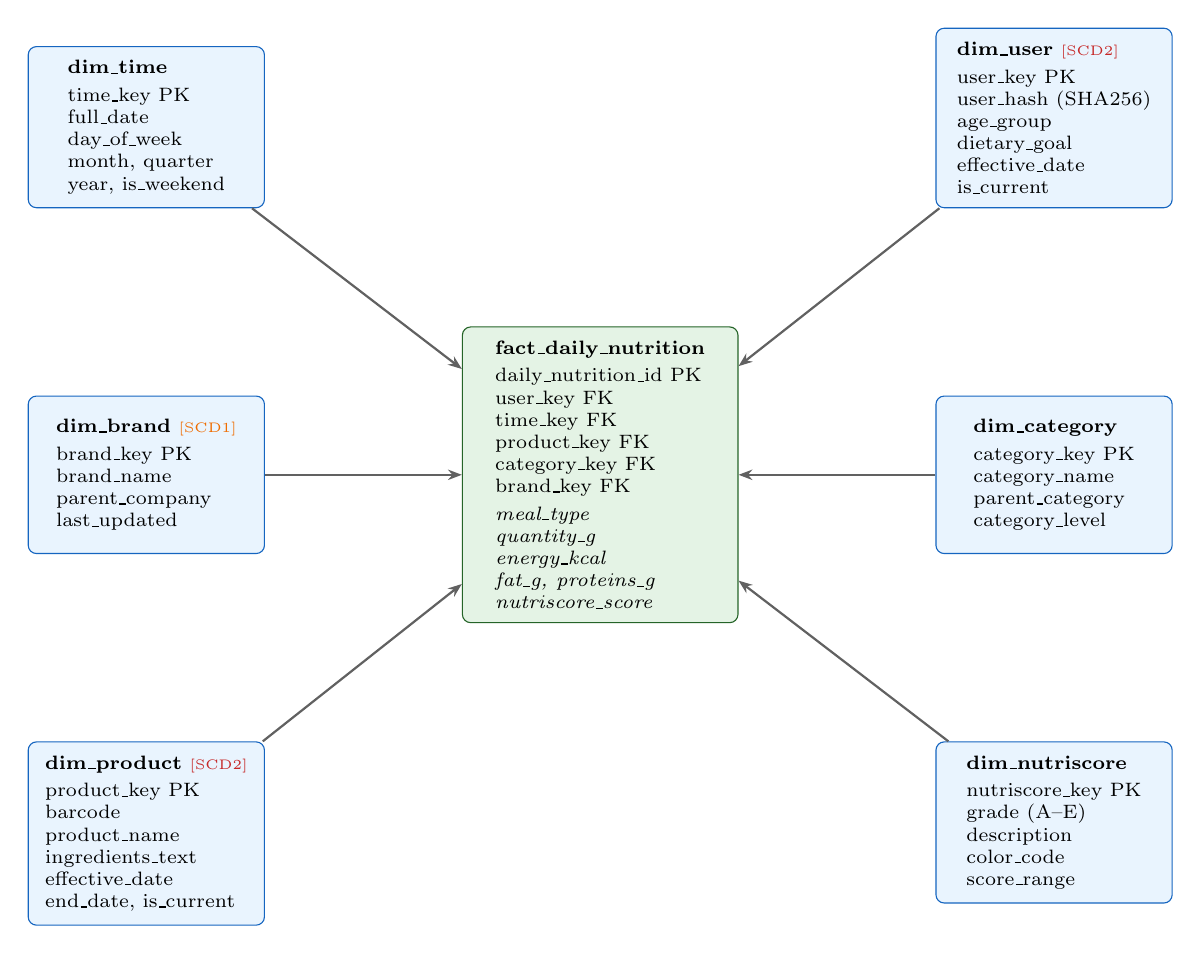
\begin{tikzpicture}[
  dim/.style={
    rectangle, rounded corners=3pt, draw=ntblue, fill=ntlightblue!20,
    minimum width=3cm, minimum height=2cm,
    font=\scriptsize, align=left, inner sep=5pt
  },
  fact/.style={
    rectangle, rounded corners=3pt, draw=ntgreen!80!black,
    fill=ntlightgreen!30, minimum width=3.5cm, minimum height=2.5cm,
    font=\scriptsize, align=left, inner sep=5pt
  },
  arr/.style={-{Stealth[length=5pt]}, thick, color=ntgray},
]

% Fact table (center)
\node[fact] (fact) {
  \textbf{fact\_daily\_nutrition}\\[2pt]
  daily\_nutrition\_id PK\\
  user\_key FK\\
  time\_key FK\\
  product\_key FK\\
  category\_key FK\\
  brand\_key FK\\[2pt]
  \textit{meal\_type}\\
  \textit{quantity\_g}\\
  \textit{energy\_kcal}\\
  \textit{fat\_g, proteins\_g}\\
  \textit{nutriscore\_score}
};

% Dimensions
\node[dim, above left=1.5cm and 2.5cm of fact] (dimtime) {
  \textbf{dim\_time}\\[2pt]
  time\_key PK\\
  full\_date\\
  day\_of\_week\\
  month, quarter\\
  year, is\_weekend
};

\node[dim, above right=1.5cm and 2.5cm of fact] (dimuser) {
  \textbf{dim\_user} {\tiny\color{ntred}[SCD2]}\\[2pt]
  user\_key PK\\
  user\_hash (SHA256)\\
  age\_group\\
  dietary\_goal\\
  effective\_date\\
  is\_current
};

\node[dim, left=2.5cm of fact] (dimbrand) {
  \textbf{dim\_brand} {\tiny\color{ntorange}[SCD1]}\\[2pt]
  brand\_key PK\\
  brand\_name\\
  parent\_company\\
  last\_updated
};

\node[dim, right=2.5cm of fact] (dimcat) {
  \textbf{dim\_category}\\[2pt]
  category\_key PK\\
  category\_name\\
  parent\_category\\
  category\_level
};

\node[dim, below left=1.5cm and 2.5cm of fact] (dimproduct) {
  \textbf{dim\_product} {\tiny\color{ntred}[SCD2]}\\[2pt]
  product\_key PK\\
  barcode\\
  product\_name\\
  ingredients\_text\\
  effective\_date\\
  end\_date, is\_current
};

\node[dim, below right=1.5cm and 2.5cm of fact] (dimns) {
  \textbf{dim\_nutriscore}\\[2pt]
  nutriscore\_key PK\\
  grade (A--E)\\
  description\\
  color\_code\\
  score\_range
};

% Arrows
\draw[arr] (dimtime) -- (fact);
\draw[arr] (dimuser) -- (fact);
\draw[arr] (dimbrand) -- (fact);
\draw[arr] (dimcat) -- (fact);
\draw[arr] (dimproduct) -- (fact);
\draw[arr] (dimns) -- (fact);

\end{tikzpicture}
\caption{Star schema --- fact\_daily\_nutrition with 6 dimensions}
\label{fig:star-schema}
\end{figure}

\subsection{Dimension and Fact Tables}

\begin{table}[H]
\centering
\caption{Data warehouse dimensions}
\label{tab:dimensions}
\begin{tabularx}{\textwidth}{L{2.5cm} C{1.5cm} C{1.2cm} L{6.5cm}}
\toprule
\textbf{Dimension} & \textbf{SCD} & \textbf{Rows} & \textbf{Description} \\
\midrule
dim\_time & --- & 4\,018 & Pre-populated time dimension (2020--2030) \\
dim\_product & Type 2 & $\sim$777K & Product attributes with history \\
dim\_brand & Type 1 & $\sim$15K & Brands (overwrite corrections) \\
dim\_category & --- & $\sim$2K & Category hierarchy \\
dim\_country & Type 3 & Ref. & Countries with expansion tracking \\
dim\_user & Type 2 & $\sim$1K & Anonymized profiles (SHA256) \\
dim\_nutriscore & --- & 5 & Nutri-Score reference (A--E) \\
\bottomrule
\end{tabularx}
\end{table}

\begin{table}[H]
\centering
\caption{Fact tables}
\label{tab:facts}
\begin{tabularx}{\textwidth}{L{3.5cm} L{4cm} L{5.5cm}}
\toprule
\textbf{Fact Table} & \textbf{Grain} & \textbf{Measures} \\
\midrule
fact\_daily\_nutrition & 1 row / user + day + product & quantity, energy, fat, proteins, carbs, fiber, salt, nutriscore, nova \\
fact\_product\_market & 1 row / product + snapshot & nutriscore, nova, ecoscore, completeness, nutrition/100g \\
\bottomrule
\end{tabularx}
\end{table}


% -----------------------------------------------------------
\section{Data Warehouse Implementation (\competence{C14})}
\label{sec:c14}
{\small\evaluation{E5} | DW creation and configuration}

\textbf{File:} \texttt{sql/init/02\_schema\_warehouse.sql} (360 lines)

The DW is implemented as a separate schema (\texttt{dw}) within the same
PostgreSQL~16 instance, created automatically during Docker Compose
initialization. Six analytical views (datamarts) are created for analyst
access: \texttt{dm\_user\_daily\_nutrition},
\texttt{dm\_product\_market\_by\_category},
\texttt{dm\_brand\_quality\_ranking},
\texttt{dm\_nutriscore\_distribution},
\texttt{dm\_nutrition\_trends},
\texttt{dm\_dw\_health}.

\textbf{Analyst access via Superset:} Superset 6.0.1 connects to the DW
via a read-only PostgreSQL role \texttt{superset} on \texttt{dw.*}.
Three dashboards provide self-service analytics.

\subsection{Test Procedure}

\begin{table}[H]
\centering
\caption{Data warehouse test procedure}
\label{tab:test-dw}
\begin{tabularx}{\textwidth}{L{3cm} L{2cm} L{7.5cm}}
\toprule
\textbf{Test} & \textbf{Scope} & \textbf{Verification} \\
\midrule
Schema creation & Technical & Tables, indexes, views created without errors \\
Dimension population & Functional & dim\_time = 4\,018 rows; dim\_nutriscore = 5 rows (A--E) \\
SCD Type 2 & Functional & Product update creates new row \texttt{is\_current=TRUE}, closes old \\
SCD Type 1 & Functional & Brand correction overwrites in place, updates \texttt{last\_updated} \\
Fact loading & Functional & Valid FK to dimensions; no orphan keys \\
Datamart views & Functional & Views return results; \texttt{nutritionist\_role} can SELECT \\
Access control & Security & \texttt{app\_readonly} cannot access \texttt{dw} schema \\
\bottomrule
\end{tabularx}
\end{table}

\subsection{Tech Stack Feedback}

\begin{table}[H]
\centering
\caption{Tech stack feedback --- Data warehouse}
\label{tab:tech-feedback}
\begin{tabularx}{\textwidth}{L{2.8cm} L{3cm} L{3.5cm} L{3.5cm}}
\toprule
\textbf{Technology} & \textbf{Project Fit} & \textbf{Advantages} & \textbf{Difficulties} \\
\midrule
PostgreSQL (OLTP+OLAP) & Good at small scale & Single instance, simple deployment & Separation needed at larger scale \\
Airflow for ETL & Industry standard & Web UI, retries, dependency mgmt & Complex setup (Celery, Redis, init) \\
PySpark ETL & Distributed-capable cleaning & Handles 800k+ rows, cluster-ready & Heavier setup than pure SQL \\
Schema isolation & Clean separation & No operational/analytical contamination & Cross-schema queries in ETL \\
\bottomrule
\end{tabularx}
\end{table}


% -----------------------------------------------------------
\section{ETL Pipelines (\competence{C15})}
\label{sec:c15}
{\small\evaluation{E5} | ETL for data warehouse input/output}

\textbf{Data formats and volumes:}
\begin{itemize}[nosep]
  \item \textbf{Input:} 798\,177 raw products from 5 sources ($\sim$4.2~GB Parquet
        + JSON + CSV), totaling $\sim$6~GB across all storage layers
  \item \textbf{Processing:} PySpark 3.5 applies 7 cleaning rules, producing
        777\,116 validated records (97.4\,\% retention)
  \item \textbf{Output:} Star schema in PostgreSQL DW (7 dimensions + 2 facts),
        Gold layer analytics in MinIO Parquet
\end{itemize}

\textbf{Pipeline overview:} 7 Airflow DAGs with 25 total tasks, orchestrated
via ExternalTaskSensor dependencies for cross-DAG coordination:

\begin{enumerate}[nosep]
  \item \texttt{etl\_datalake\_ingest} --- Ingest raw data to bronze layer
  \item \texttt{etl\_aggregate\_clean} --- PySpark cleaning (bronze $\to$ silver)
  \item \texttt{etl\_import\_to\_db} --- Load cleaned data to operational DB
  \item \texttt{etl\_load\_warehouse} --- Populate star schema (dimensions + facts)
  \item \texttt{etl\_gold\_aggregates} --- Generate gold analytics (silver $\to$ gold)
  \item \texttt{etl\_data\_quality} --- Run 6 quality checks
  \item \texttt{etl\_backup\_maintenance} --- Weekly backups + cleanup
\end{enumerate}

\subsection{ETL Workflow}

\begin{figure}[H]
\centering
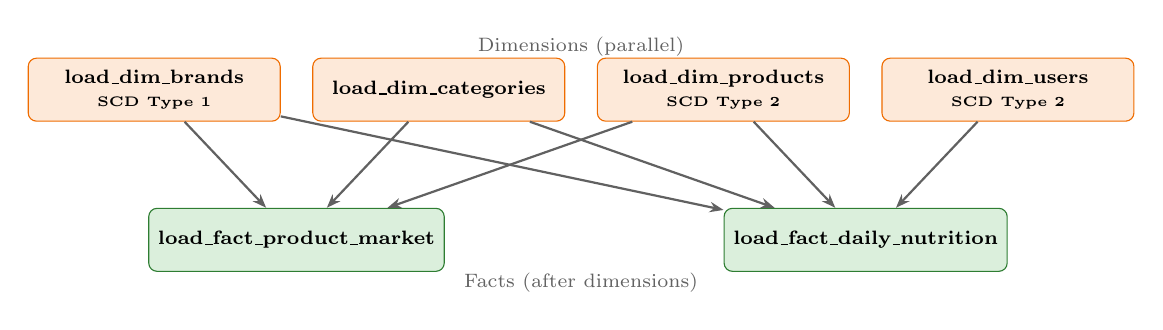
\begin{tikzpicture}[
  task/.style={
    rectangle, rounded corners=3pt, draw=ntorange, fill=ntorange!15,
    minimum width=3.2cm, minimum height=0.8cm,
    font=\scriptsize\bfseries, align=center
  },
  arr/.style={-{Stealth[length=5pt]}, thick, color=ntgray},
]

% Dimension tasks (parallel)
\node[task] (brands) {load\_dim\_brands\\{\tiny SCD Type 1}};
\node[task, right=0.4cm of brands] (cats) {load\_dim\_categories};
\node[task, right=0.4cm of cats] (prods) {load\_dim\_products\\{\tiny SCD Type 2}};
\node[task, right=0.4cm of prods] (users) {load\_dim\_users\\{\tiny SCD Type 2}};

% Fact tasks
\node[task, below=1.5cm of $(brands)!0.5!(cats)$, fill=ntlightgreen!40, draw=ntgreen] (factmarket) {load\_fact\_product\_market};
\node[task, below=1.5cm of $(prods)!0.5!(users)$, fill=ntlightgreen!40, draw=ntgreen] (factnutri) {load\_fact\_daily\_nutrition};

% Arrows
\draw[arr] (brands) -- (factmarket);
\draw[arr] (cats) -- (factmarket);
\draw[arr] (prods) -- (factmarket);
\draw[arr] (prods) -- (factnutri);
\draw[arr] (users) -- (factnutri);
\draw[arr] (cats) -- (factnutri);
\draw[arr] (brands) -- (factnutri);

% Labels
\node[font=\scriptsize\color{ntgray}, above=0.3cm of $(cats)!0.5!(prods)$]
  {Dimensions (parallel)};
\node[font=\scriptsize\color{ntgray}, below=0.3cm of $(factmarket)!0.5!(factnutri)$]
  {Facts (after dimensions)};
\end{tikzpicture}
\caption{ETL DAG dependencies --- \texttt{etl\_load\_warehouse}}
\label{fig:etl-dag}
\end{figure}


% -----------------------------------------------------------
\section{DW Maintenance and Monitoring (\competence{C16})}
\label{sec:c16}
{\small\evaluation{E6} | Administration and supervision}

\subsection{Activity Logging}

The \texttt{app.etl\_activity\_log} table provides structured logging
with three alert categories:

\begin{table}[H]
\centering
\caption{ETL activity log schema}
\label{tab:activity-log}
\begin{tabularx}{\textwidth}{L{3cm} L{2.5cm} L{7cm}}
\toprule
\textbf{Column} & \textbf{Type} & \textbf{Description} \\
\midrule
log\_id & SERIAL PK & Auto-incrementing identifier \\
log\_timestamp & TIMESTAMP & Event occurrence time \\
alert\_category & VARCHAR(20) & \texttt{CRITICAL}, \texttt{WARNING}, or \texttt{INFO} \\
dag\_id & VARCHAR(100) & Airflow DAG identifier \\
task\_id & VARCHAR(100) & Airflow task identifier \\
event\_type & VARCHAR(50) & \texttt{task\_failure}, \texttt{task\_success}, \texttt{sla\_miss}, etc. \\
message & TEXT & Human-readable event description \\
details & JSONB & Structured metadata (duration, record counts, errors) \\
acknowledged & BOOLEAN & Whether incident has been acknowledged \\
\bottomrule
\end{tabularx}
\end{table}

\textbf{Historical seed data:} Migration \texttt{002\_seed\_etl\_activity\_log.sql}
populates approximately 20 log entries spanning 14 days, covering
successful ETL runs, transient failures with retry recovery, backup
completions, SLA misses, and data quality alerts. This demonstrates
ongoing monitoring throughout the project lifecycle (\competence{C6}).

\subsection{Alert System --- MailHog SMTP}

Airflow DAGs are configured with email alerts on failure, delivered via
MailHog SMTP (a development-mode mail server):

\begin{lstlisting}[language=Python, caption={Alerting default configuration (airflow/plugins/alerting.py)}]
ALERTING_DEFAULT_ARGS = {
    "email_on_failure": True,
    "email_on_retry": False,
    "email": ["admin@nutritrack.local"],
    "retries": 2,
    "retry_delay": timedelta(minutes=5),
}
\end{lstlisting}

\textbf{MailHog configuration} in \texttt{docker-compose.yml}:

\begin{lstlisting}[language=bash, caption={MailHog service and Airflow SMTP configuration}]
# MailHog service (port 8025 for web UI)
mailhog:
  image: mailhog/mailhog:latest
  ports:
    - "1025:1025"   # SMTP
    - "8025:8025"   # Web UI

# Airflow SMTP settings (environment variables)
AIRFLOW__SMTP__SMTP_HOST: mailhog
AIRFLOW__SMTP__SMTP_PORT: "1025"
AIRFLOW__SMTP__SMTP_STARTTLS: "false"
AIRFLOW__SMTP__SMTP_SSL: "false"
AIRFLOW__SMTP__SMTP_MAIL_FROM: airflow@nutritrack.local
\end{lstlisting}

When a task fails after the configured number of retries, an email alert
is sent to \texttt{admin@nutritrack.local} and can be verified in the
MailHog web interface at port~8025. The alerting plugin also logs every
alert, retry and SLA miss to the \texttt{app.etl\_activity\_log} table
for persistent tracking.

\subsection{Service Level Indicators (SLA)}

\begin{table}[H]
\centering
\caption{Service level indicators}
\label{tab:sla}
\begin{tabularx}{\textwidth}{L{4cm} C{2cm} L{6.5cm}}
\toprule
\textbf{Indicator} & \textbf{Target} & \textbf{Measurement} \\
\midrule
ETL success rate & $>$~95\,\% & Airflow DAG run history \\
Data freshness & $<$~24h & Last successful run timestamp \\
DW query response time & $<$~5s & EXPLAIN ANALYZE on datamart views \\
Backup success rate & 100\,\% & Backup log entries \\
Data completeness & $>$~80\,\% & Cleaning report statistics \\
\bottomrule
\end{tabularx}
\end{table}

\subsection{Maintenance Task Prioritization (ITIL-Aligned)}

Maintenance tasks follow a four-tier priority matrix inspired by
ITIL\,v4 incident management.

\begin{table}[H]
\centering
\caption{Maintenance priority matrix (P1--P4)}
\label{tab:priority-matrix}
\begin{tabularx}{\textwidth}{C{1.2cm} C{1.5cm} C{1.8cm} C{2cm} L{5cm}}
\toprule
\textbf{Priority} & \textbf{Severity} & \textbf{Response} & \textbf{Resolution} & \textbf{Examples} \\
\midrule
P1 & Critical & $<$~1h & $<$~4h & ETL failure blocking analytics; DB corruption; backup failure; security breach \\
P2 & High & $<$~4h & $<$~8h & SLA breach (ETL $<$~95\,\%); data freshness $>$~24h; repeated DAG failure \\
P3 & Medium & $<$~24h & $<$~3 days & Non-critical DAG failure; slow queries ($>$~5s); dashboard errors \\
P4 & Low & Next sprint & Next release & Doc updates; cosmetic changes; new datamart requests \\
\bottomrule
\end{tabularx}
\end{table}

\textbf{Assignment rules:}
\begin{itemize}[nosep]
  \item \textbf{P1:} Assigned to on-call engineer immediately.
        Escalate to project lead after 2\,h.
  \item \textbf{P2:} Assigned during business hours.
        Escalate after 4\,h.
  \item \textbf{P3:} Triaged in daily standup, assigned to next
        available engineer.
  \item \textbf{P4:} Added to sprint backlog, prioritized during
        sprint planning.
\end{itemize}

\textbf{Escalation path:}
L1~(Engineer) $\to$ L2~(Senior Engineer, if unresolved within response
time) $\to$ L3~(Project Lead, P1$>$2h or P2$>$4h).

\subsection{SLA Compliance Dashboard (Grafana)}

A dedicated Grafana dashboard (\texttt{monitoring/grafana/dashboards/sla-compliance.json})
provides real-time visibility into all service level indicators:

\begin{table}[H]
\centering
\caption{SLA dashboard panels (10 panels)}
\label{tab:sla-dashboard}
\begin{tabularx}{\textwidth}{L{4cm} C{2cm} L{6.5cm}}
\toprule
\textbf{Panel} & \textbf{Target} & \textbf{Prometheus Source} \\
\midrule
Overall SLA Compliance & $>$~95\,\% & Weighted composite of all indicators \\
ETL Success Rate & $>$~95\,\% & \texttt{airflow\_dagrun\_duration\_*} \\
Data Freshness & $<$~24h & \texttt{airflow\_dagrun\_start\_timestamp} \\
Backup Completion & 100\,\% & \texttt{airflow\_ti\_successes} (7d) \\
Query Response Time & $<$~5s & \texttt{pg\_stat\_activity\_max\_tx\_duration} \\
Storage Usage & $<$~85\,\% & \texttt{pg\_database\_size\_bytes} \\
ETL Success Rate (7d) & $>$~95\,\% & 7-day trend chart of DAG runs \\
DAG Run Outcomes (7d) & --- & Stacked bar: success/failure/retry \\
Active Alerts Count & 0 & Count of \texttt{CRITICAL} entries in activity log \\
Data Quality Score & $>$~90\,\% & Cleaning report completeness metrics \\
\bottomrule
\end{tabularx}
\end{table}

The dashboard enables proactive identification of degrading performance
before SLA breaches occur, with 7-day trend charts for ETL success rate
and DAG run outcomes.

\subsection{Backup Procedures}

\textbf{Full backup:} \texttt{make backup} (complete database)\\
\textbf{Partial backup:} \texttt{make backup-dw} (DW schema only)\\
Format: \texttt{pg\_dump --format=custom --compress=6}, optional upload
to MinIO.

\textbf{Scheduled backups:} The \texttt{etl\_backup\_maintenance} DAG
runs weekly and includes tasks for DW schema backup, storage health
checks, and cleanup of old backup files.


\subsection{New Source Integration Procedure}

When a new data source must be integrated into the platform, the following
6-step procedure is applied:

\begin{enumerate}[nosep]
  \item \textbf{Source assessment:} Document the new source in the data
        topography --- format (JSON, CSV, Parquet, API), volume, update
        frequency, access method, license, and \rgpd{} implications.
  \item \textbf{Extraction script:} Create a new extraction script following
        the standard structure (entry point, dependency init, connection
        config, business logic, error handling, result saving). Add to
        Git with documentation.
  \item \textbf{Bronze ingestion:} Configure a new Airflow DAG (or add tasks
        to an existing DAG) to upload raw data to MinIO bronze bucket under
        a new prefix (\texttt{new\_source/\{ds\}/*.format}).
  \item \textbf{Silver transformation:} Update the PySpark cleaning pipeline
        to include the new source. Add source-specific cleaning rules if needed.
        Update the schema mapping configuration.
  \item \textbf{DW integration:} Add or update dimension and fact table
        loading tasks in \texttt{etl\_load\_warehouse} DAG. If new dimensions
        are required, create migration scripts and update the star schema.
  \item \textbf{Validation and monitoring:} Add data quality checks for the
        new source. Configure alerting for the new DAG tasks. Update the
        data catalog metadata in MinIO. Run end-to-end test.
\end{enumerate}

\subsection{New Access Creation Procedure}

To grant a new user or group access to the data warehouse or data lake:

\begin{enumerate}[nosep]
  \item \textbf{Define access scope:} Identify which schemas (app, dw),
        tables, and MinIO buckets the new user/group needs. Apply the
        principle of least privilege. Document in the access rights matrix
        (Table~\ref{tab:access-matrix}).
  \item \textbf{Configure database access:} Create a PostgreSQL role with
        appropriate permissions:
        \begin{lstlisting}[language=SQL, numbers=none, frame=none, xleftmargin=0em, framexleftmargin=0em]
-- Example: new analyst role
CREATE ROLE new_analyst_role LOGIN PASSWORD 'secure_pwd';
GRANT USAGE ON SCHEMA dw TO new_analyst_role;
GRANT SELECT ON ALL TABLES IN SCHEMA dw TO new_analyst_role;
        \end{lstlisting}
  \item \textbf{Configure data lake access:} Create a MinIO policy scoped
        to the required buckets and apply it to the user/group:
        \begin{lstlisting}[language=bash, numbers=none, frame=none, xleftmargin=0em, framexleftmargin=0em]
# Example: read-only access to gold bucket
mc admin policy create myminio gold-readonly gold-policy.json
mc admin user add myminio new_analyst secure_pwd
mc admin policy attach myminio gold-readonly --user new_analyst
        \end{lstlisting}
\end{enumerate}

\subsection{Scalability Documentation}

\begin{table}[H]
\centering
\caption{Scalability procedures for platform evolution}
\label{tab:scalability}
\begin{tabularx}{\textwidth}{L{3cm} L{3cm} L{6.5cm}}
\toprule
\textbf{Dimension} & \textbf{Current State} & \textbf{Scaling Procedure} \\
\midrule
Storage space & PostgreSQL: $\sim$2~GB; MinIO: $\sim$4~GB & PostgreSQL: add tablespaces on new volumes. MinIO: add storage nodes to the cluster (erasure coding supports 4--16 nodes). Docker volume resize via host filesystem. \\
New datamarts & 6 analytical views & Create new SQL view in \texttt{dw} schema; grant SELECT to target role; add to Superset as dataset; document in data catalog. \\
Compute capacity & Single Docker host & Migrate to Docker Swarm or Kubernetes for horizontal scaling. Airflow: switch from CeleryExecutor to KubernetesExecutor. PySpark: connect to a standalone or YARN cluster. \\
New data sources & 5 sources & Follow the 6-step new source integration procedure above. \\
Additional users & 4 role groups & Follow the 3-step new access creation procedure above. \\
\bottomrule
\end{tabularx}
\end{table}

\subsection{\rgpd{} Registry and Sorting Procedures (C16)}

The personal data registry (Table~\ref{tab:rgpd}) is maintained and updated
whenever new data categories are introduced. Sorting and deletion procedures
are automated:

\begin{itemize}[nosep]
  \item \textbf{Automated sorting:} The \texttt{rgpd\_cleanup\_expired\_data()}
        function runs monthly (scheduled via Airflow) and performs:
        (1)~deletion of meal records older than 2 years,
        (2)~deactivation of user accounts past 3-year retention,
        (3)~logging of all deletions to the activity log.
  \item \textbf{Manual right-to-deletion:} Upon user request, an admin can
        execute \texttt{DELETE FROM app.users WHERE user\_id = \$UUID} which
        cascades to all associated meals and meal items.
  \item \textbf{Data lake compliance:} No personal data is stored in the data
        lake. MinIO lifecycle rules enforce automatic deletion of bronze data
        at 90 days and backups at 30 days.
\end{itemize}


% -----------------------------------------------------------
\section{SCD Dimension Variations (\competence{C17})}
\label{sec:c17}
{\small\evaluation{E6} | Kimball Type 1, 2, 3}

\begin{figure}[H]
\centering
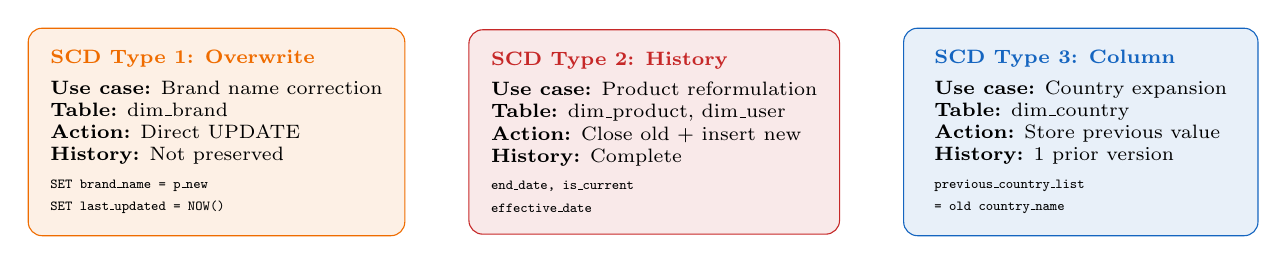
\begin{tikzpicture}[
  scd/.style={
    rectangle, rounded corners=5pt, draw=#1, fill=#1!10,
    minimum width=4.5cm, minimum height=2.5cm,
    font=\scriptsize, align=left, inner sep=8pt
  },
  title/.style={font=\small\bfseries\color{#1}},
]

% SCD Type 1
\node[scd=ntorange] (scd1) at (0,0) {
  \textbf{\color{ntorange}SCD Type 1: Overwrite}\\[3pt]
  \textbf{Use case:} Brand name correction\\
  \textbf{Table:} dim\_brand\\
  \textbf{Action:} Direct UPDATE\\
  \textbf{History:} Not preserved\\[2pt]
  {\tiny \texttt{SET brand\_name = p\_new}}\\
  {\tiny \texttt{SET last\_updated = NOW()}}
};

% SCD Type 2
\node[scd=ntred, right=0.8cm of scd1] (scd2) {
  \textbf{\color{ntred}SCD Type 2: History}\\[3pt]
  \textbf{Use case:} Product reformulation\\
  \textbf{Table:} dim\_product, dim\_user\\
  \textbf{Action:} Close old + insert new\\
  \textbf{History:} Complete\\[2pt]
  {\tiny \texttt{end\_date, is\_current}}\\
  {\tiny \texttt{effective\_date}}
};

% SCD Type 3
\node[scd=ntblue, right=0.8cm of scd2] (scd3) {
  \textbf{\color{ntblue}SCD Type 3: Column}\\[3pt]
  \textbf{Use case:} Country expansion\\
  \textbf{Table:} dim\_country\\
  \textbf{Action:} Store previous value\\
  \textbf{History:} 1 prior version\\[2pt]
  {\tiny \texttt{previous\_country\_list}}\\
  {\tiny \texttt{= old country\_name}}
};

\end{tikzpicture}
\caption{Three Slowly Changing Dimension types implemented}
\label{fig:scd-types}
\end{figure}


% =============================================================
% BLOCK 4: DATA LAKE
% =============================================================
\chapter{Block 4 --- Data Lake}
\label{ch:bloc4}

% -----------------------------------------------------------
\section{Data Lake Architecture (\competence{C18})}
\label{sec:c18}
{\small\evaluation{E7} | Architecture design}

\subsection{Medallion Architecture}

\begin{figure}[H]
\centering
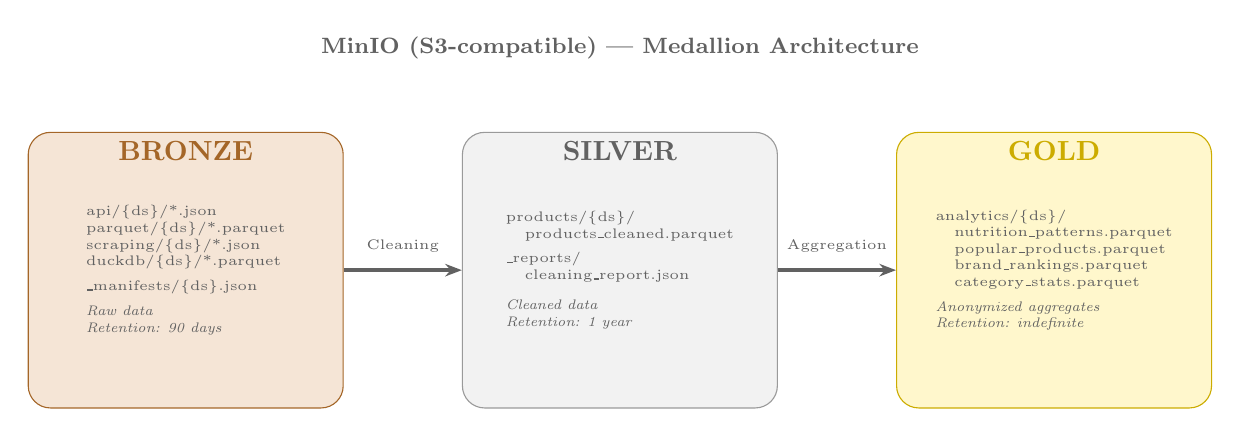
\begin{tikzpicture}[
  layer/.style={
    rectangle, rounded corners=8pt, draw=#1!80!black, fill=#1!20,
    minimum width=4cm, minimum height=3.5cm,
    font=\small, align=center, inner sep=10pt
  },
  arr/.style={-{Stealth[length=6pt]}, very thick, color=ntgray},
  content/.style={font=\tiny, align=left, text=ntgray},
]

% Bronze
\node[layer=bronze] (br) {};
\node[font=\bfseries\color{bronze!80!black}, anchor=north] at (br.north)
  {BRONZE};
\node[content, anchor=center] at (br.center) {
  api/\{ds\}/*.json\\
  parquet/\{ds\}/*.parquet\\
  scraping/\{ds\}/*.json\\
  duckdb/\{ds\}/*.parquet\\[3pt]
  \_manifests/\{ds\}.json\\[3pt]
  \textit{Raw data}\\
  \textit{Retention: 90 days}
};

% Silver
\node[layer=silver, right=1.5cm of br] (sv) {};
\node[font=\bfseries\color{ntgray}, anchor=north] at (sv.north) {SILVER};
\node[content, anchor=center] at (sv.center) {
  products/\{ds\}/\\
  \quad products\_cleaned.parquet\\[3pt]
  \_reports/\\
  \quad cleaning\_report.json\\[5pt]
  \textit{Cleaned data}\\
  \textit{Retention: 1 year}
};

% Gold
\node[layer=gold, right=1.5cm of sv] (gd) {};
\node[font=\bfseries\color{gold!80!black}, anchor=north] at (gd.north)
  {GOLD};
\node[content, anchor=center] at (gd.center) {
  analytics/\{ds\}/\\
  \quad nutrition\_patterns.parquet\\
  \quad popular\_products.parquet\\
  \quad brand\_rankings.parquet\\
  \quad category\_stats.parquet\\[3pt]
  \textit{Anonymized aggregates}\\
  \textit{Retention: indefinite}
};

% Arrows
\draw[arr] (br) -- (sv);
\draw[arr] (sv) -- (gd);

% Labels
\node[font=\tiny\color{ntgray}, above=0.1cm of $(br)!0.5!(sv)$] {Cleaning};
\node[font=\tiny\color{ntgray}, above=0.1cm of $(sv)!0.5!(gd)$] {Aggregation};

% MinIO label
\node[font=\footnotesize\bfseries\color{ntgray},
      above=0.8cm of sv] {MinIO (S3-compatible) --- Medallion Architecture};

\end{tikzpicture}
\caption{Data lake medallion architecture (Bronze / Silver / Gold)}
\label{fig:medallion}
\end{figure}

\subsection{Addressing the 3~V's}

\begin{table}[H]
\centering
\caption{Volume, Velocity, Variety constraints and solutions}
\label{tab:3v}
\begin{tabularx}{\textwidth}{C{1.5cm} L{4cm} L{7.5cm}}
\toprule
\textbf{V} & \textbf{Challenge} & \textbf{Solution} \\
\midrule
Volume & 3M+ products ($\sim$5\,GB Parquet) & DuckDB reads Parquet without memory loading; MinIO scales to petabytes \\
Variety & JSON, Parquet, CSV, SQL & Bronze stores raw formats; Silver normalizes to unified Parquet \\
Velocity & Daily API updates, weekly bulk & Airflow DAGs on schedule; Bronze preserves snapshots by \{ds\}/ \\
\bottomrule
\end{tabularx}
\end{table}

\subsection{Catalog Tool Comparison}

\begin{table}[H]
\centering
\caption{Catalog tool comparison and selection}
\label{tab:catalog-compare}
\begin{tabularx}{\textwidth}{L{2.5cm} C{2.5cm} C{2.5cm} C{3.5cm}}
\toprule
\textbf{Criterion} & \textbf{Apache Atlas} & \textbf{DataHub} & \textbf{JSON Catalog} \\
\midrule
Complexity & High & Medium & \textbf{Low} \\
Setup time & Days & Hours & \textbf{Minutes} \\
Integration & Hadoop & REST API & \textbf{MinIO native} \\
Resource cost & High (JVM) & Medium & \textbf{Minimal} \\
\bottomrule
\end{tabularx}
\end{table}

\textbf{Selection:} Custom JSON catalog --- chosen for its minimal
overhead, direct MinIO integration, and sufficiency at project scale.


% -----------------------------------------------------------
\section{Infrastructure Components (\competence{C19})}
\label{sec:c19}
{\small\evaluation{E7} | Installation and configuration}

The entire infrastructure is deployable in a development environment
via Docker Compose. The installation has been tested on macOS (Apple Silicon)
and Linux (Ubuntu 22.04) without errors.

\textbf{Prerequisites:} Docker Engine 24+, Docker Compose v2, 8~GB RAM minimum,
10~GB free disk space.

\begin{lstlisting}[language=bash, caption={Infrastructure deployment}]
# Clone repository
git clone https://github.com/Reetika12795/NutriTrack.git
cd nutritrack

# Full platform startup
docker compose up -d

# Verify service health
docker compose ps
# Expected output: 15 services running

# Makefile commands for testing
make up            # Start all services
make pipeline      # Run extraction -> cleaning -> import
make setup-lake    # Initialize MinIO buckets
make lake-status   # Check storage status
\end{lstlisting}

\textbf{Service inventory (15 services):}

\begin{table}[H]
\centering
\caption{Docker Compose service inventory}
\label{tab:services}
\begin{tabularx}{\textwidth}{C{0.5cm} L{3cm} L{2.5cm} C{1.5cm} L{4.5cm}}
\toprule
\textbf{\#} & \textbf{Service} & \textbf{Image} & \textbf{Port} & \textbf{Purpose} \\
\midrule
1 & PostgreSQL & postgres:16-alpine & 5432 & OLTP + OLAP database \\
2 & Redis & redis:7-alpine & 6379 & Cache + Celery broker \\
3 & MinIO & minio/minio:latest & 9000/9001 & S3-compatible object storage \\
4 & Airflow Webserver & custom (Python 3.11) & 8080 & ETL web interface \\
5 & Airflow Scheduler & custom (Python 3.11) & --- & DAG scheduling \\
6 & Airflow Worker & custom (Python 3.11) & --- & Task execution (Celery) \\
7 & Airflow Init & custom (Python 3.11) & --- & DB migration + user creation \\
8 & FastAPI & custom (Python 3.11) & 8000 & REST API \\
9 & Streamlit & custom (Python 3.11) & 8501 & Frontend UI \\
10 & Prometheus & prom/prometheus & 9090 & Metrics collection \\
11 & Grafana & grafana/grafana & 3000 & Dashboards + alerting \\
12 & MailHog & mailhog/mailhog & 8025 & Dev email server \\
13 & postgres-exporter & prometheuscommunity & 9187 & PostgreSQL metrics \\
14 & MinIO createbuckets & minio/mc & --- & Bucket initialization \\
15 & Superset & custom (Python 3.9) & 8088 & BI dashboards \\
\bottomrule
\end{tabularx}
\end{table}

\textbf{Storage system configuration:}
\begin{itemize}[nosep]
  \item \textbf{PostgreSQL:} 4 schemas (\texttt{app}, \texttt{raw}, \texttt{staging},
        \texttt{dw}), initialized via SQL migration scripts in \texttt{sql/init/}
  \item \textbf{MinIO:} 4 buckets (\texttt{bronze}, \texttt{silver}, \texttt{gold},
        \texttt{backups}), created automatically by the \texttt{createbuckets}
        init container with lifecycle rules applied
  \item \textbf{Redis:} In-memory cache for Airflow Celery broker and API
        session management
\end{itemize}

\textbf{Batch and real-time tools:}
\begin{itemize}[nosep]
  \item \textbf{Batch:} Airflow DAGs (7 DAGs, 25 tasks) orchestrate all
        ETL workflows on configurable schedules (daily, weekly)
  \item \textbf{Real-time:} FastAPI provides synchronous query access to
        the database; Streamlit provides real-time dashboard updates
  \item \textbf{Catalog:} The JSON catalog in MinIO is connected to the
        storage system and updated automatically by ETL pipelines
\end{itemize}


% -----------------------------------------------------------
\section{Data Catalog Management (\competence{C20})}
\label{sec:c20}
{\small\evaluation{E7} | Catalog, lifecycle and monitoring}

The data catalog is stored as \texttt{\_catalog/metadata.json} in each
MinIO bucket, updated daily by the ETL pipeline. It documents for each
dataset: description, format, update frequency, source, schema, owner,
quality and lineage.

\subsection{Feed Method per Source}

\begin{table}[H]
\centering
\caption{Feed method selection per data source}
\label{tab:feed-methods}
\begin{tabularx}{\textwidth}{L{2.5cm} L{2cm} L{3cm} L{5cm}}
\toprule
\textbf{Source} & \textbf{Method} & \textbf{Frequency} & \textbf{Justification} \\
\midrule
OFF REST API & Batch (API pull) & Daily & Limited to category-based queries; rate-limited; suitable for incremental updates \\
OFF Parquet & Batch (file download) & Weekly & Full dataset refresh; 4.2~GB file too large for frequent downloads \\
ANSES/EFSA & Batch (scraping) & Monthly & Reference values change rarely; respectful crawling \\
PostgreSQL (app) & Batch (SQL extract) & Daily & Extract new/modified records since last run via \texttt{updated\_at} timestamp \\
DuckDB analytics & On-demand & As needed & Analytical queries triggered by user request or scheduled report \\
\bottomrule
\end{tabularx}
\end{table}

\subsection{Catalog Metadata Updates}

The data catalog metadata is updated at each ETL run through the following process:
\begin{enumerate}[nosep]
  \item Each DAG task writes a manifest file (\texttt{\_manifests/\{ds\}.json})
        containing: source, record count, file sizes, schema hash, and timestamp.
  \item The catalog update task aggregates manifests and updates
        \texttt{\_catalog/metadata.json} with: last update time, total records,
        schema version, data lineage (source $\to$ bronze $\to$ silver $\to$ gold),
        and quality metrics from the cleaning report.
  \item The Streamlit data catalog browser provides a read-only UI for exploring
        catalog metadata, dataset schemas, and lineage.
\end{enumerate}

\subsection{Lifecycle-Based Deletion and Update Procedures}

\begin{table}[H]
\centering
\caption{Data lifecycle rules per bucket}
\label{tab:lifecycle}
\begin{tabularx}{\textwidth}{L{2cm} L{2cm} L{3cm} L{5.5cm}}
\toprule
\textbf{Bucket} & \textbf{Retention} & \textbf{Deletion Method} & \textbf{Procedure} \\
\midrule
Bronze & 90 days & MinIO lifecycle rule & Automatic expiration; old snapshots deleted after 90 days to free storage \\
Silver & 1 year & Manual / lifecycle & Outdated cleaned datasets replaced by new runs; old versions expire after 1 year \\
Gold & Indefinite & Manual only & Aggregated analytics retained indefinitely; deletion requires admin approval \\
Backups & 30 days & MinIO lifecycle rule & Old backups automatically purged; most recent 4 weekly backups always retained \\
\bottomrule
\end{tabularx}
\end{table}

\textbf{Update procedures:}
\begin{itemize}[nosep]
  \item \textbf{Data refresh:} New ETL runs write to date-partitioned paths
        (\texttt{\{ds\}/}), preserving previous versions until lifecycle expiration.
  \item \textbf{Schema evolution:} If the source schema changes, the cleaning pipeline
        is updated, a new schema version is recorded in the catalog, and old silver
        data is marked as deprecated.
  \item \textbf{Regulatory deletion:} For \rgpd{} compliance, any personal data
        inadvertently ingested into bronze is immediately deleted and logged
        as a CRITICAL event in the activity log.
\end{itemize}

\subsection{Monitoring with Alerts}

The data lake is monitored through Prometheus metrics and Grafana dashboards
with automated alerting:

\begin{table}[H]
\centering
\caption{Data lake monitoring --- alerts and thresholds}
\label{tab:lake-monitoring}
\begin{tabularx}{\textwidth}{L{3.5cm} C{2cm} L{3cm} L{4cm}}
\toprule
\textbf{Metric} & \textbf{Threshold} & \textbf{Alert Channel} & \textbf{Action} \\
\midrule
MinIO disk usage & $>$~85\,\% & Grafana $\to$ MailHog & Trigger lifecycle cleanup; expand storage \\
MinIO server status & DOWN & Grafana $\to$ MailHog & Restart container; escalate if persistent \\
ETL feed failure & 2 consecutive & Airflow $\to$ MailHog & Retry; check source availability; log CRITICAL \\
Catalog update age & $>$~48h & Grafana $\to$ MailHog & Investigate ETL pipeline; check DAG scheduler \\
Bronze data volume & $>$~10~GB & Grafana panel & Review lifecycle rules; archive old snapshots \\
Memory usage & $>$~90\,\% & Grafana $\to$ MailHog & Scale compute; optimize PySpark memory settings \\
\bottomrule
\end{tabularx}
\end{table}

Grafana alert rules are defined in \texttt{monitoring/grafana/provisioning/alerting/}
and configured to send notifications via MailHog SMTP for development
and via email/Slack for production deployment.


% -----------------------------------------------------------
\section{Data Governance (\competence{C21})}
\label{sec:c21}
{\small\evaluation{E7} | Governance rules and access control}

\begin{table}[H]
\centering
\caption{Access rights matrix by group}
\label{tab:access-matrix}
\begin{tabularx}{\textwidth}{L{2.5cm} L{2.5cm} L{3.5cm} C{1.5cm} L{3cm}}
\toprule
\textbf{Group} & \textbf{PG Role} & \textbf{MinIO Policy} & \textbf{API Role} & \textbf{Description} \\
\midrule
Users & app\_readonly & gold: read & user & Search, meals \\
Nutritionists & nutritionist\_role & silver+gold: read & nutritionist & Cleaned data \\
Administrators & admin\_role & all: write & admin & Full access \\
ETL Service & etl\_service & bronze/silver/gold: write & --- & Automated pipeline \\
\bottomrule
\end{tabularx}
\end{table}

\textbf{Governance principles:}
\begin{itemize}[nosep]
  \item Rights applied to groups (not individuals) when possible
  \item Access limited to necessary resources per group (least privilege)
  \item No personal data in the data lake
  \item Gold bucket publicly readable for anonymous analytics
  \item All access changes documented and logged
\end{itemize}

\subsection{Groups and Rights Documentation}

\begin{table}[H]
\centering
\caption{Detailed access rights per group and resource}
\label{tab:detailed-rights}
\begin{tabularx}{\textwidth}{L{2.2cm} L{2.5cm} C{1.5cm} C{1.5cm} C{1.5cm} C{1.5cm}}
\toprule
\textbf{Resource} & \textbf{Permission} & \textbf{Users} & \textbf{Nutri.} & \textbf{Admin} & \textbf{ETL} \\
\midrule
PG: app schema & SELECT & Yes & Yes & Yes & Yes \\
PG: app schema & INSERT/UPDATE & --- & --- & Yes & Yes \\
PG: dw schema & SELECT & --- & Yes & Yes & Yes \\
PG: dw schema & INSERT/UPDATE & --- & --- & Yes & Yes \\
PG: staging schema & ALL & --- & --- & Yes & Yes \\
MinIO: bronze & READ & --- & --- & Yes & Yes \\
MinIO: bronze & WRITE & --- & --- & Yes & Yes \\
MinIO: silver & READ & --- & Yes & Yes & Yes \\
MinIO: silver & WRITE & --- & --- & Yes & Yes \\
MinIO: gold & READ & Yes & Yes & Yes & Yes \\
MinIO: gold & WRITE & --- & --- & Yes & Yes \\
MinIO: backups & READ/WRITE & --- & --- & Yes & Yes \\
API endpoints & Public (/register, /login) & Yes & Yes & Yes & --- \\
API endpoints & Authenticated (/products, /meals) & Yes & Yes & Yes & --- \\
API endpoints & Admin (/admin/*) & --- & --- & Yes & --- \\
Airflow UI & View DAGs & --- & --- & Yes & Yes \\
Grafana & View dashboards & --- & Yes & Yes & --- \\
\bottomrule
\end{tabularx}
\end{table}

\textbf{Access update procedures:}
\begin{itemize}[nosep]
  \item \textbf{Adding a user to a group:} Assign the appropriate PostgreSQL role
        (\texttt{GRANT role\_name TO username}) and MinIO policy
        (\texttt{mc admin policy attach}). Update the access matrix documentation.
  \item \textbf{Removing access:} Revoke PostgreSQL role (\texttt{REVOKE role\_name
        FROM username}) and detach MinIO policy. Log the change.
  \item \textbf{Audit:} Quarterly review of all access grants against the access
        matrix to ensure compliance with least-privilege principle and \rgpd{}
        requirements.
\end{itemize}


% =============================================================
% CI/CD AND DOCUMENTATION
% =============================================================
\chapter{CI/CD and Documentation}
\label{ch:cicd}

\section{GitHub Actions Workflows}
\label{sec:cicd-docs}

Four CI/CD workflows are configured in \texttt{.github/workflows/} and
run on every push and pull request to \texttt{main}:

\begin{table}[H]
\centering
\caption{CI/CD workflow summary}
\label{tab:cicd}
\begin{tabularx}{\textwidth}{L{3cm} L{3cm} L{7cm}}
\toprule
\textbf{Workflow} & \textbf{Trigger} & \textbf{Description} \\
\midrule
\texttt{test.yml} & Push/PR to main & Runs \texttt{pytest tests/ -v} with Python~3.11 \\
\texttt{lint.yml} & Push/PR to main & Runs \texttt{ruff check} + \texttt{ruff format --check} (Python) and \texttt{sqlfluff lint} (SQL) \\
\texttt{docker.yml} & Push/PR to main & Validates Docker Compose configuration \\
\texttt{deploy-docs.yml} & Push to main (mkdocs paths) & Builds MkDocs site and deploys to GitHub Pages \\
\bottomrule
\end{tabularx}
\end{table}

\section{MkDocs Documentation Site}

A comprehensive documentation site is built with MkDocs Material and
deployed automatically to GitHub Pages at
\url{https://reetika12795.github.io/NutriTrack/}. The site covers:

\begin{itemize}[nosep]
  \item \textbf{Architecture:} System overview, data flow pipeline,
        infrastructure details
  \item \textbf{Data Warehouse:} Star schema, ETL pipelines, SCD
        implementation, datamarts
  \item \textbf{Data Lake:} Medallion architecture, data catalog,
        governance and \rgpd{}
  \item \textbf{API:} REST API reference
  \item \textbf{Monitoring:} Alerting system (MailHog + activity log),
        SLA dashboard (Grafana)
  \item \textbf{Certification:} Competency matrix, audit report
\end{itemize}

The documentation source lives in \texttt{mkdocs/} and is automatically
rebuilt and deployed via the \texttt{deploy-docs.yml} GitHub Actions
workflow on every change to the \texttt{mkdocs/} directory.


% =============================================================
% CONCLUSION
% =============================================================
\chapter{Conclusion}
\label{ch:conclusion}

\section{Demo Plan}

The live demo follows this sequence (32~minutes):

\begin{table}[H]
\centering
\caption{Live demo plan}
\label{tab:demo-plan}
\begin{tabularx}{\textwidth}{C{1cm} C{1.5cm} L{9.5cm}}
\toprule
\textbf{Step} & \textbf{Duration} & \textbf{Demonstration} \\
\midrule
1 & 3 min & Launch \texttt{docker compose up -d}, verify 15 services \\
2 & 5 min & Full pipeline execution: extraction $\rightarrow$ cleaning $\rightarrow$ import \\
3 & 3 min & Airflow interface: DAG history, logs, dependencies \\
4 & 3 min & PostgreSQL: \texttt{app} schema, SQL queries, GIN index \\
5 & 4 min & REST API: Swagger UI, registration, JWT login, search, alternatives \\
6 & 3 min & Streamlit: product search, meal logging, nutrition summary \\
7 & 3 min & Data warehouse: \texttt{dw} schema, star schema, datamart views \\
8 & 3 min & SCD: product reformulation simulation (Type~2), brand correction (Type~1) \\
9 & 3 min & MinIO Console: bronze/silver/gold buckets, catalog, lifecycle \\
10 & 2 min & Governance: access matrix, MinIO policies, \rgpd{} \\
\bottomrule
\end{tabularx}
\end{table}


\section{Competency-to-Artifact Verification Matrix}

\begin{longtable}{C{1cm} C{1cm} L{5cm} L{5cm}}
\toprule
\textbf{Comp.} & \textbf{Eval.} & \textbf{Artifacts} & \textbf{Section} \\
\midrule
\endhead
C1 & E1, E2 & Interview grids, synthesis note (RICE, feasibility, pre-project) & \S\ref{sec:e1}, \S\ref{sec:e2} \\
C2 & E2 & Topography (4 parts: glossary, models, flows, access), flux matrix & \S\ref{sec:e2} \\
C3 & E2 & Architecture study, CAPEX, risks, eco-responsibility & \S\ref{sec:e2} \\
C4 & E2 & Airflow monitoring, extraction\_log, veille newsletter & \S\ref{sec:e2} \\
C5 & E3 & Roadmap, Gantt calendar, team, budget, poker planning & \S\ref{sec:e3} \\
C6 & E2, E3 & Makefile, Airflow UI, indicators, activity log & \S\ref{sec:e2}, \S\ref{sec:e3} \\
C7 & E3 & Communication strategy, onboarding, feedback collection & \S\ref{sec:e3} \\
C8 & E4 & 5 extraction scripts (API, Parquet, scraping, DB, DuckDB) & \S\ref{sec:c8} \\
C9 & E4 & 7 SQL queries with optimizations & \S\ref{sec:c9} \\
C10 & E4 & PySpark pipeline (798K $\to$ 777K), 6 quality checks & \S\ref{sec:c10}, \S\ref{sec:dq} \\
C11 & E4 & MCD/MLD/MPD, \rgpd{} registry, import & \S\ref{sec:c11} \\
C12 & E4 & FastAPI 8 endpoints, JWT HS256, 3 roles, OpenAPI docs & \S\ref{sec:c12} \\
C13 & E5 & Star schema (2 facts, 7 dimensions), bottom-up justified & \S\ref{sec:c13} \\
C14 & E5 & DW creation, access config, tests, tech stack feedback & \S\ref{sec:c14} \\
C15 & E5 & 7 Airflow DAGs, 25 tasks, PySpark ETL logic & \S\ref{sec:c15} \\
C16 & E6 & Activity log, alerts, SLA, ITIL, backups, new source/access procedures, scalability & \S\ref{sec:c16} \\
C17 & E6 & SCD Type 1/2/3 with examples & \S\ref{sec:c17} \\
C18 & E7 & Medallion architecture, 3V, catalog comparison & \S\ref{sec:c18} \\
C19 & E7 & 15-service Docker Compose, MinIO, Airflow, installation tested & \S\ref{sec:c19} \\
C20 & E7 & Catalog, feed methods, lifecycle, monitoring with alerts & \S\ref{sec:c20} \\
C21 & E7 & RBAC, group policies, detailed rights matrix, \rgpd{} & \S\ref{sec:c21} \\
\bottomrule
\end{longtable}


\section{Lessons Learned}

\begin{enumerate}[nosep]
  \item \textbf{Single PostgreSQL for OLTP+OLAP} works at small scale
        thanks to schema isolation, but would require separation at
        larger scale.
  \item \textbf{DuckDB} is remarkably effective for big data analytics
        without dedicated infrastructure.
  \item \textbf{Airflow CeleryExecutor} adds complexity but enables
        ETL parallelism.
  \item \textbf{SCD Type~2} requires careful \texttt{IS DISTINCT FROM}
        logic for NULL values.
  \item \textbf{\rgpd{} compliance} must be designed in from the start,
        not retrofitted.
  \item \textbf{CI/CD pipelines} (GitHub Actions for lint, test, docker,
        docs deployment) catch regressions early and automate
        documentation publishing.
\end{enumerate}


\section{Future Improvements}

\begin{itemize}[nosep]
  \item Separate OLTP/OLAP with a dedicated analytical engine
        (ClickHouse, Redshift)
  \item Migrate to a full data catalog (DataHub)
  \item Extend data quality framework (6 formal checks already implemented
        and logged to \texttt{staging.data\_quality\_checks}; next step:
        integrate Great Expectations for schema-level validation)
  \item Real-time streaming with Apache Kafka
  \item Advanced monitoring with PagerDuty integration
  \item Machine learning recommendation engine in the gold layer
\end{itemize}


% =============================================================
% BIBLIOGRAPHY
% =============================================================
\begin{thebibliography}{99}

\bibitem{off}
Open Food Facts.
\textit{Open Food Facts --- The free food products database}.
\url{https://world.openfoodfacts.org/}, 2024.

\bibitem{kimball}
R.~Kimball and M.~Ross.
\textit{The Data Warehouse Toolkit: The Definitive Guide to Dimensional
Modeling}. 3rd edition, Wiley, 2013.

\bibitem{eu1169}
Regulation (EU) No~1169/2011.
\textit{Provision of food information to consumers}.
Official Journal of the European Union, 2011.

\bibitem{gdpr}
Regulation (EU) 2016/679.
\textit{General Data Protection Regulation (GDPR)}.
Official Journal of the European Union, 2016.

\bibitem{rgesn}
Direction interministerielle du numerique.
\textit{Referentiel general d'ecoconception de services numeriques
(RGESN)}.
\url{https://ecoresponsable.numerique.gouv.fr/publications/referentiel-general-ecoconception/}, 2024.

\bibitem{airflow}
Apache Software Foundation.
\textit{Apache Airflow Documentation}.
\url{https://airflow.apache.org/docs/}, 2024.

\bibitem{fastapi}
S.~Ramirez.
\textit{FastAPI --- Modern, fast web framework for building APIs with Python}.
\url{https://fastapi.tiangolo.com/}, 2024.

\bibitem{duckdb}
M.~Raasveldt and H.~Muhleisen.
\textit{DuckDB: An Embeddable Analytical Database}.
Proc. SIGMOD, 2019.

\bibitem{minio}
MinIO, Inc.
\textit{MinIO --- High Performance Object Storage}.
\url{https://min.io/}, 2024.

\bibitem{anses}
ANSES.
\textit{Nutritional reference values}.
\url{https://www.anses.fr/fr/content/les-references-nutritionnelles-en-vitamines-et-mineraux}, 2024.

\end{thebibliography}


\end{document}
